% CINF200 - Plantilla LaTeX de informe académico tipo paper
% Universidad Andrés Bello - Ingeniería Civil Informática

\documentclass[11pt,a4paper]{article}

\usepackage[utf8]{inputenc}
\usepackage[T1]{fontenc}
% Se omite babel para mantener compatibilidad con instalaciones mínimas de TeX.
\usepackage{lmodern}
\usepackage{geometry}
\geometry{top=2.2cm,bottom=2.0cm,left=2.3cm,right=2.3cm,headheight=22pt}
\usepackage{graphicx}
\usepackage{xcolor}
\usepackage{booktabs}
\usepackage{array}
\usepackage{longtable}
\usepackage{tabularx}
\usepackage{enumitem}
\usepackage{amsmath,amssymb}
\usepackage{caption}
\usepackage{float}
\usepackage{fancyhdr}
\usepackage{titlesec}
\usepackage{hyperref}
\usepackage{cleveref}
\usepackage{pgfgantt}
\usepackage{colortbl}
\usepackage{tikz}
\usetikzlibrary{arrows.meta,positioning,shapes.geometric,fit,backgrounds,decorations.pathreplacing}

% Bibliografía numérica, ordenada por aparición, mediante BibTeX.
% Compilación: pdflatex -> bibtex -> pdflatex -> pdflatex.

\definecolor{CINFBlue}{HTML}{17365D}
\definecolor{CINFNavy}{HTML}{111827}
\definecolor{CINFRed}{HTML}{B4202A}
\definecolor{CINFGray}{HTML}{5B6573}

\hypersetup{
  colorlinks=true,
  linkcolor=CINFBlue,
  citecolor=CINFRed,
  urlcolor=CINFBlue,
  pdftitle={Sistema de Detección de Anomalías en Tráfico IoT mediante Machine Learning},
  pdfauthor={Felipe Vergara Rodríguez - Universidad Andrés Bello}
}

\pagestyle{fancy}
\fancyhf{}
\lhead{\footnotesize\textcolor{CINFGray}{Detección de Anomalías en Tráfico IoT mediante ML | Ingeniería Civil Informática}}
\rfoot{\footnotesize\textcolor{CINFGray}{\thepage}}
\renewcommand{\headrulewidth}{0.3pt}
\renewcommand{\headrule}{\hbox to\headwidth{\color{CINFBlue}\leaders\hrule height \headrulewidth\hfill}}

\titleformat{\section}{\Large\bfseries\color{CINFBlue}}{\thesection.}{0.6em}{}
\titleformat{\subsection}{\large\bfseries\color{CINFBlue}}{\thesubsection}{0.6em}{}
\titleformat{\subsubsection}{\normalsize\bfseries\color{CINFNavy}}{\thesubsubsection}{0.6em}{}
\titlespacing*{\section}{0pt}{2.0ex plus .3ex minus .2ex}{0.8ex}
\titlespacing*{\subsection}{0pt}{1.5ex plus .2ex minus .2ex}{0.5ex}

\setlist[itemize]{leftmargin=1.7em,itemsep=0.2em,topsep=0.2em}
\setlist[enumerate]{leftmargin=1.9em,itemsep=0.2em,topsep=0.2em}
\setlength{\parindent}{0pt}
\setlength{\parskip}{0.55em}
\emergencystretch=2em
\captionsetup{font=small,labelfont=bf,labelsep=period}

% Nombres en español para índices y bibliografía (la plantilla omite babel).
\renewcommand{\contentsname}{Índice}
\renewcommand{\listtablename}{Índice de tablas}
\renewcommand{\listfigurename}{Índice de figuras}
\renewcommand{\tablename}{Tabla}
\renewcommand{\figurename}{Figura}
\renewcommand{\refname}{Referencias}

% Datos del proyecto
\newcommand{\projecttitle}{Sistema de Detección de Anomalías en Tráfico IoT mediante Machine Learning}
\newcommand{\students}{Felipe Vergara Rodríguez}
\newcommand{\advisor}{Nicolás Caselli Benavente}
\newcommand{\institution}{Universidad Andrés Bello}
\newcommand{\degree}{Ingeniería Civil Informática}

\begin{document}

% -----------------------------------------------------------------------------
% PORTADA Y METADATOS
% -----------------------------------------------------------------------------
\begin{titlepage}
\thispagestyle{empty}
\begin{center}
\IfFileExists{logo_ici.png}{
\includegraphics[width=0.82\textwidth]{logo_ici.png}}{}

\vspace{1.0cm}
{\large\color{CINFRed}\textbf{ARTÍCULO DE INVESTIGACIÓN TECNOLÓGICA APLICADA}}\\[0.3cm]
{\LARGE\color{CINFNavy}\textbf{\projecttitle}}\\[0.25cm]
{\large\color{CINFGray}Ingeniería Civil Informática · Facultad de Ingeniería}

\vspace{1.0cm}
\renewcommand{\arraystretch}{1.25}
\begin{tabular}{>{\bfseries}p{4.0cm}p{8.0cm}}
Autor & \students\\
Profesor guía & \advisor\\
Institución & \institution --- Sede Viña del Mar\\
Carrera & \degree\\
Periodo & Segundo Semestre 2026 (Noviembre 2026)\\
\end{tabular}
\end{center}
\end{titlepage}

% -----------------------------------------------------------------------------
% RESUMEN E ÍNDICES
% -----------------------------------------------------------------------------
\begin{abstract}
La masificación de dispositivos del Internet de las Cosas (IoT) con recursos limitados dificulta detectar tráfico de botnets sin instalar agentes locales ni generar falsas alarmas. Este proyecto implementa y evalúa un sistema centralizado de detección de anomalías en tráfico IoT basado en Machine Learning liviano, estructurado bajo una metodología híbrida que integra el ciclo de ciencia de datos CRISP-DM con prácticas de aseguramiento de calidad CRISP-ML(Q) y gestión iterativa Scrum. Se auditó íntegramente el conjunto UCI N-BaIoT (nueve dispositivos comerciales, 89 archivos CSV, 7.062.606 registros y 115 características), identificando y neutralizando una fuga de laboratorio en las columnas de media y varianza de jitter que codificaban la época Unix de captura. Se implementó una arquitectura de doble pipeline (offline y online) con defensa en tres anillos, consola MVP en Streamlit protegida con autenticación JWT HS256, verificación criptográfica SHA-256, persistencia SQLite parametrizada, incorporación dinámica de nuevos equipos (Modo Aprendizaje 24h e invitados) y 25 pruebas automatizadas. La evaluación incluye una referencia histórica frente a línea base y un protocolo riguroso de 73 experimentos con separación 6/2/1 de dispositivos, bloques posicionales disjuntos y exclusión de familias de ataque. Random Forest obtiene un F1 medio de 0,9995 (FPR medio de 0,14\% y latencia de 5,28 ms) ante dispositivos excluidos con familias conocidas; sin embargo, al excluir completamente Mirai en el dispositivo 4, el recall desciende a 39,90\%. Estos hallazgos delimitan con rigor el alcance real del enfoque supervisado y orientan la continuidad experimental en hardware de borde.
\end{abstract}

\textbf{Palabras clave:} Machine Learning; Internet de las Cosas (IoT); detección de intrusiones; ciberseguridad; botnets; CRISP-DM.

\clearpage
\tableofcontents
\listoftables
\listoffigures
\clearpage

% -----------------------------------------------------------------------------
% CUERPO DEL INFORME
% -----------------------------------------------------------------------------
\section{Introducción}
La masificación de dispositivos conectados a internet —sensores, cámaras, relés inteligentes y asistentes domésticos— ha transformado la forma en que los hogares interactúan con la tecnología. Sin embargo, esta adopción acelerada no ha ido acompañada de un nivel equivalente de seguridad: los dispositivos IoT suelen priorizar bajo costo y bajo consumo energético, dejando de lado mecanismos robustos de protección frente a intrusiones.

Esta debilidad ha sido explotada históricamente por ataques de tipo botnet, que comprometen múltiples dispositivos de forma simultánea para ejecutar ataques a mayor escala. Detectar este tipo de comportamiento anómalo de manera oportuna es un desafío relevante tanto para usuarios domésticos como para pequeñas organizaciones que no cuentan con herramientas de monitoreo especializadas.

El presente proyecto propone abordar este problema mediante el uso de Machine Learning supervisado, entrenando y comparando distintos modelos de clasificación capaces de distinguir tráfico de red normal de tráfico malicioso, con el fin de sentar las bases de una herramienta accesible de detección temprana para redes IoT domésticas.

\section{Problema y fundamentación}
Los dispositivos IoT domésticos (sensores, relés inteligentes, cámaras, asistentes conectados) suelen priorizar bajo costo y bajo consumo energético por sobre la seguridad, lo que los convierte en el eslabón más débil de una red doméstica. A diferencia de un computador o smartphone, rara vez cuentan con antivirus, actualizaciones automáticas robustas, o mecanismos de detección de intrusos adaptados a sus recursos limitados de procesamiento y memoria.

\subsection{Diagnóstico, necesidad y contexto}
El proyecto se orienta a usuarios domésticos con redes de dispositivos IoT propias, un escenario cada vez más común dada la masificación de hogares inteligentes en Chile y el mundo. Este contexto es representativo de miles de redes domésticas que carecen de herramientas de monitoreo de seguridad accesibles.

\textbf{Causas del problema:}
\begin{itemize}
    \item Firmware con configuraciones por defecto (contraseñas débiles, puertos abiertos).
    \item Comunicación sin cifrar en varios dispositivos de bajo costo.
    \item Ausencia de sistemas de detección diseñados específicamente para el perfil de tráfico IoT, distinto al de un computador convencional.
\end{itemize}

\textbf{Efectos del problema:}
\begin{itemize}
    \item Los dispositivos comprometidos pueden integrarse a redes de bots (\textit{botnets}); el caso histórico más relevante es Mirai, uno de los botnets utilizados para generar el tráfico de ataque documentado en el dataset N-BaIoT \cite{meidan2018}.
    \item Riesgo de pivoteo: un atacante ingresa por el dispositivo más débil y luego compromete otros equipos de la misma red.
    \item Pérdida de confianza del usuario final en la adopción de tecnología IoT.
\end{itemize}

\textbf{Oportunidad tecnológica:} existen datasets públicos con tráfico real de ataques a dispositivos IoT (N-BaIoT, IoT-23, BoT-IoT) que permiten entrenar modelos de Machine Learning capaces de identificar patrones anómalos a partir de patrones estadísticos; su transferencia a ataques desconocidos requiere evaluación específica. Esto representa una oportunidad concreta de aplicar Machine Learning a un problema vigente y de alto impacto en ciberseguridad.

\subsection{Pregunta de investigación o desafío de ingeniería}
¿Cómo cambia el desempeño de clasificadores clásicos de tráfico IoT al separar los dispositivos de ajuste, calibración y prueba y excluir familias de botnets, y qué limitaciones impiden trasladar sus resultados a una red operacional? La comparación con Deep Learning se limita a antecedentes bibliográficos; no constituye un experimento controlado de este avance.

\subsection{Pertinencia tecnológica y valor organizacional}
La solución propuesta se justifica porque aborda un problema real y creciente (la vulnerabilidad de los dispositivos IoT domésticos frente a ataques de botnet) mediante una técnica actualmente vigente y con evidencia sólida en la literatura: el uso de Machine Learning supervisado para detección de anomalías en tráfico de red. A diferencia de los sistemas de seguridad tradicionales basados en firmas (que solo detectan ataques ya conocidos), un modelo entrenado con Machine Learning puede aprender patrones estadísticos del tráfico; la detección de variantes no observadas es una hipótesis que se evalúa, no una capacidad garantizada.

Además, la comparación de al menos cuatro modelos distintos (Random Forest, SVM, Regresión Logística y Gradient Boosting) permite fundamentar la elección final del modelo no solo en su exactitud, sino también en su viabilidad de despliegue en entornos de bajos recursos, lo que hace la solución más realista y aplicable a dispositivos IoT reales.

El principal beneficiario es el usuario doméstico o la pequeña organización que gestiona una red de dispositivos IoT sin contar con personal ni herramientas especializadas en ciberseguridad. Actualmente, este tipo de usuarios no tiene forma accesible de saber si uno de sus dispositivos está comprometido o siendo utilizado como parte de una botnet. El dashboard desarrollado como parte del MVP ofrece al analista una visualización experimental de predicciones sobre un catálogo de prueba; todavía no se ha evaluado su comprensión con usuarios ni su eficacia en una red real.

El proyecto se enmarca dentro de la tendencia de transformación digital orientada a la ciberseguridad proactiva: en lugar de reaccionar frente a un ataque ya consumado, el sistema propuesto habilita una toma de decisiones informada y temprana, alertando al usuario u organización sobre comportamiento anómalo antes de que el impacto sea mayor. Esto es consistente con el enfoque de seguridad moderno basado en monitoreo continuo y análisis de datos, en lugar de reglas estáticas.

\subsection{Factibilidad, responsabilidad y riesgos}
\textbf{Datos y restricciones:} el proyecto utilizará el dataset público N-BaIoT \cite{nbaiot-dataset}, disponible de forma gratuita en el repositorio de UCI Machine Learning, por lo que no existen restricciones de acceso ni costos asociados a la obtención de datos. Como restricción relevante, el dataset fue capturado en 2018 sobre un conjunto acotado de nueve dispositivos comerciales, por lo que no representa necesariamente el comportamiento de tráfico de dispositivos IoT más recientes; esto se reconoce como una limitación de representatividad temporal, no como un riesgo de privacidad, dado que los datos no contienen información personal de usuarios reales, solo tráfico de red a nivel de paquetes.

\textbf{Riesgos técnicos:}
\begin{itemize}
    \item \textit{Sobreajuste (overfitting):} al comparar cuatro modelos sobre un mismo dataset, existe el riesgo de que uno memorice patrones específicos en lugar de generalizar. \textit{Mitigación:} validación cruzada y separación clara entre conjuntos de entrenamiento y prueba.
    \item \textit{Desbalance de clases:} el tráfico de ataque puede estar sobre o subrepresentado respecto al normal. \textit{Mitigación:} técnicas de balanceo (\textit{undersampling}/\textit{oversampling}) durante el preprocesamiento.
    \item \textit{Brecha entre datos de laboratorio y tráfico real:} el MVP se probará con tráfico simulado o capturado en un entorno controlado, que puede no replicar la complejidad de una red real. \textit{Mitigación:} declarar explícitamente esta limitación en las conclusiones.
\end{itemize}

\textbf{Riesgos organizacionales:} al tratarse de un prototipo de investigación sin despliegue en una red productiva, el principal riesgo es sobreestimar la aplicabilidad inmediata del sistema. \textit{Mitigación:} delimitar explícitamente que el sistema corresponde a un MVP de validación experimental, no a un producto de seguridad en producción.

\textbf{Privacidad:} el dataset no contiene información personal identificable; corresponde a metadatos de tráfico de red (tamaños de paquete, tiempos, protocolos). \textit{Mitigación ante un escenario real:} procesar los datos de forma local, sin enviarlos a servidores externos, e informar al usuario qué se analiza y con qué fin.

\textbf{Sesgos:} el dataset fue capturado sobre nueve dispositivos comerciales específicos, por lo que el modelo puede aprender patrones particulares de esos dispositivos en lugar de un patrón general. \textit{Mitigación:} declarar esta limitación de representatividad al reportar resultados.

\textbf{Explicabilidad:} al priorizar Machine Learning clásico por sobre Deep Learning, modelos como Random Forest y Gradient Boosting permiten obtener la importancia relativa de cada característica (\textit{feature importance}), lo que posibilita explicar por qué el sistema clasificó un tráfico como malicioso.

\textbf{Impactos:} el principal impacto esperado es positivo, al dotar a usuarios sin conocimientos técnicos de una herramienta accesible de detección. Un sistema con falsos positivos frecuentes podría generar desconfianza; por ello la comparación de precisión y recall entre modelos busca minimizar este efecto.

\section{Objetivos}

\subsection{Objetivo general}
Implementar y evaluar un modelo de Machine Learning liviano para la detección de anomalías y tráfico malicioso asociado a ataques de botnet en redes de dispositivos IoT, utilizando datasets públicos de tráfico real y validando su funcionamiento en un escenario de demostración controlado.

\subsection{Objetivos específicos}
\begin{itemize}
  \item Analizar el estado del arte en detección de intrusiones para IoT, comparando enfoques de Machine Learning clásico y Deep Learning en cuanto a desempeño y viabilidad computacional.
  \item Procesar y preparar el dataset N-BaIoT, aplicando limpieza, selección de características (\textit{feature engineering}) y balanceo de clases entre tráfico normal y malicioso.
  \item Implementar y comparar al menos cuatro modelos de clasificación supervisada ya establecidos en la literatura (Random Forest, Support Vector Machine, Regresión Logística y Gradient Boosting), midiendo su desempeño mediante precisión, recall, F1-score, tiempo de entrenamiento y tiempo de inferencia, a fin de seleccionar aquel con la mejor relación entre desempeño y costo computacional. Como línea base se utilizará un clasificador simple (Regresión Logística sin ajuste de hiperparámetros), y se distinguirá la validación cruzada histórica sobre entrenamiento de la evaluación externa por dispositivos y familias excluidas.
  \item Evaluar la capacidad de generalización del modelo seleccionado frente a dispositivos no vistos durante el entrenamiento, mediante una estrategia de validación por dispositivo excluido (\textit{leave-one-device-out}), contrastando este resultado con el obtenido en la evaluación estándar.
  \item Diseñar y construir un escenario de demostración controlado que reproduzca tráfico de red normal y malicioso mediante reproducción de vectores CSV etiquetados, permitiendo comprobar el recorrido funcional sin atribuirle equivalencia con tráfico en producción.
  \item Implementar un dashboard web simple (desarrollado en Streamlit) que consuma el escenario de demostración y visualice en tiempo real la clasificación entregada por el modelo, junto con importancia global de características y desviaciones locales, distinguiéndolas de explicaciones causales.
\end{itemize}

\section{Estado del arte y antecedentes}
La literatura reciente en detección de intrusiones para IoT se concentra mayoritariamente en el uso del dataset N-BaIoT, un conjunto de datos de tráfico real capturado desde nueve dispositivos IoT comerciales infectados con los botnets Mirai y BASHLITE \cite{meidan2018}. La Tabla \ref{tab:estado-arte} presenta una comparación de los principales enfoques encontrados.

\begin{table}[H]
\centering
\caption{Comparación de enfoques en detección de botnets IoT mediante Machine Learning.}
\label{tab:estado-arte}
\small
\begin{tabularx}{\textwidth}{p{2.1cm}p{2.4cm}p{1.6cm}X X}
\toprule
\textbf{Autor / Año} & \textbf{Método} & \textbf{Dataset} & \textbf{Resultado} & \textbf{Limitación reconocida} \\
\midrule
Meidan et al., 2018 \cite{meidan2018} & Autoencoders profundos & N-BaIoT & Evaluación mediante exactitud, precisión, recall y F1-score sobre dispositivos comerciales reales & Modelos entrenados por dispositivo individual, dificulta escalar \\
Catillo et al., 2022 \cite{allinone2022} & Autoencoder único combinado & N-BaIoT & Buenos resultados por dispositivo individual & Transferencia a otras redes no evaluada en este proyecto \\
Hossain e Islam, 2023 \cite{hossain2023} & Selección de características híbrida + ensemble (Extra Trees) & N-BaIoT y otros & $\sim$99,99\% de exactitud & Evaluación mayormente offline sobre datasets estáticos \\
Naeem et al., 2025 \cite{cnnbilstm2025} & Híbrido CNN + BiLSTM con atención & N-BaIoT & $\sim$99\% de exactitud, alta precisión y recall & No comparado experimentalmente bajo los recursos de este proyecto \\
Wardana et al., 2024 \cite{ensembledn} & DNN con ensamblaje entre dispositivos & N-BaIoT & 97,21\% de exactitud (recall 87,31\%) & Heterogeneidad entre fabricantes dificulta generalizar un solo modelo \\
Bhilwarawala et al., 2026 \cite{bridge2026} & Benchmark heterogéneo y arquitectura multirrama (TCH-Net) & Múltiples dominios IoT & Evidencia brechas severas de desempeño al cambiar de dominio & Confirma que las métricas intra-dominio sobreestiman la generalización real \\
\bottomrule
\end{tabularx}
\end{table}

\textbf{Síntesis crítica y brecha identificada:} los antecedentes muestran alternativas clásicas y profundas con resultados altos, pero sus métricas no son directamente comparables sin controlar datos, particiones y recursos. El trabajo de Wardana et al.\ \cite{ensembledn} reporta 97,21\% de exactitud y 87,31\% de recall, mientras que Bhilwarawala et al.\ \cite{bridge2026} advierten caídas relevantes al evaluar transferencia entre dominios heterogéneos; esas cifras ilustran por qué la exactitud aislada sobre particiones aleatorias no basta. La contribución del proyecto consiste en evaluar explícitamente dispositivos y familias excluidas bajo un protocolo sanitizado y documentar con honestidad las fallas de transferencia. No se demuestra aquí superioridad frente a Deep Learning ni se afirma que un replay resuelva la brecha de producción.

\section{Metodología}

\subsection{Enfoque metodológico híbrido: CRISP-DM / CRISP-ML(Q) y Scrum}
Dado que el proyecto articula simultáneamente un ciclo de investigación en ciencia de datos e inteligencia artificial (auditoría del dataset, ingeniería de características y evaluación experimental de modelos) con el desarrollo incremental de un producto de software de ciberseguridad (consola MVP, control de acceso y persistencia SQL), se adoptó un \textbf{marco metodológico híbrido de doble capa}:
\begin{enumerate}
  \item \textbf{Capa científica y de ciclo de vida de datos (CRISP-DM complementada con CRISP-ML(Q)):} se adopta el estándar industrial \textit{Cross-Industry Standard Process for Data Mining} (CRISP-DM) \cite{chapman2000crispdm} en sus seis fases iterativas (comprensión del negocio, comprensión de los datos, preparación, modelado, evaluación y despliegue), extendido con los principios de aseguramiento de calidad de \textbf{CRISP-ML(Q)} \cite{studer2021crispmlq}. Esta extensión es determinante para el problema IoT porque exige verificar explícitamente la ausencia de fuga de datos (\textit{data leakage}), evaluar robustez ante desplazamientos de distribución (\textit{zero-day}), preservar integridad criptográfica de artefactos (\texttt{SHA-256}) y establecer monitoreo continuo en la fase de despliegue.
  \item \textbf{Capa de gestión ágil y desarrollo incremental (Scrum adaptado):} para gobernar la ejecución temporal, la trazabilidad de entregables y la gestión de riesgos, se emplea una adaptación de \textbf{Scrum} \cite{schwaber2020scrum} organizada en \textit{Sprints} de tres a cuatro semanas con \textit{Product Backlog}, criterios de terminado (\textit{Definition of Done}: código versionado, 25 pruebas unitarias en verde, artefactos firmados y documentación sincronizada) y revisiones periódicas con el docente guía en rol de \textit{Product Owner} técnico.
\end{enumerate}

La Figura~\ref{fig:metodologia-hibrida} ilustra la articulación entre ambas capas y la Tabla~\ref{tab:crisp-scrum} mapea cada fase de CRISP-DM/CRISP-ML(Q) con los Sprints ejecutados en 2026-2 (Sprints 1 a 3) y proyectados para la continuidad 2027-1 (Sprints 4 a 7).

\begin{figure}[H]
\centering
\resizebox{\textwidth}{!}{%
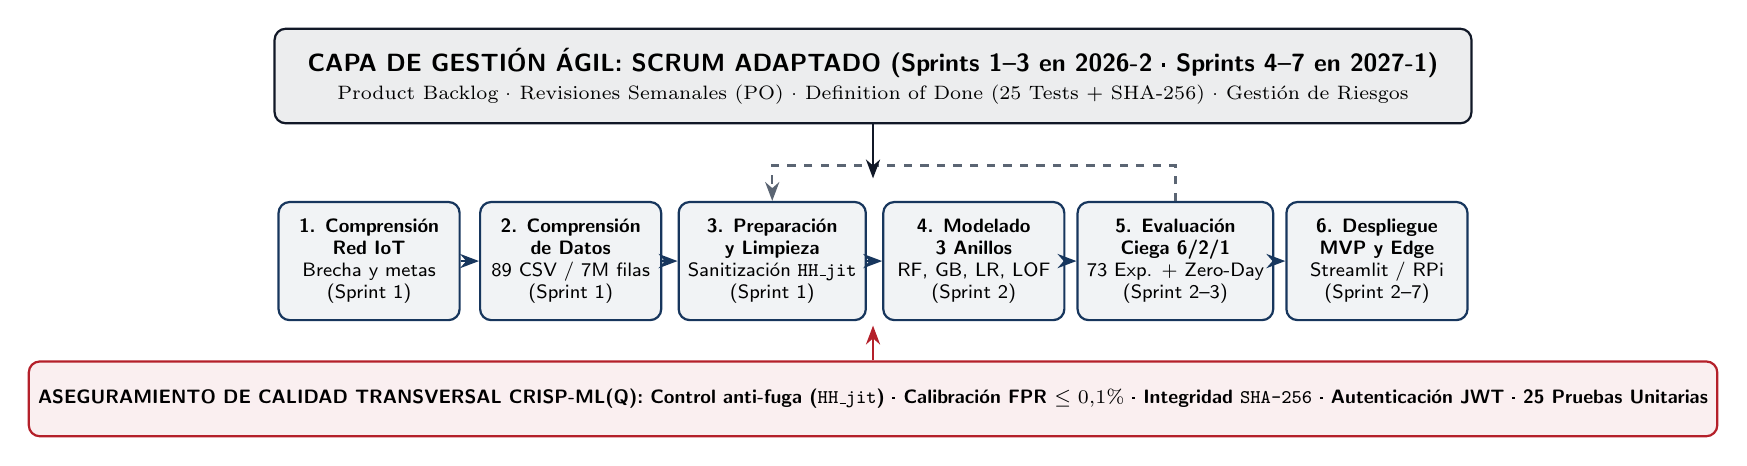
\begin{tikzpicture}[
  scrumbox/.style={rectangle, draw=CINFNavy, fill=CINFNavy!8, thick, rounded corners=4pt, minimum width=15.2cm, minimum height=1.2cm, align=center, font=\small\bfseries\sffamily},
  phase/.style={rectangle, draw=CINFBlue, fill=CINFBlue!6, thick, rounded corners=4pt, minimum width=2.3cm, minimum height=1.5cm, align=center, font=\scriptsize\sffamily},
  qbar/.style={rectangle, draw=CINFRed, fill=CINFRed!7, thick, rounded corners=4pt, minimum width=15.2cm, minimum height=0.95cm, align=center, font=\scriptsize\bfseries\sffamily},
  arr/.style={-{Stealth[length=2.4mm]}, thick, CINFBlue}
]
  \node[scrumbox] (scrum) at (0, 2.35) {CAPA DE GESTIÓN ÁGIL: SCRUM ADAPTADO (Sprints 1--3 en 2026-2 · Sprints 4--7 en 2027-1)\\[-1pt]\scriptsize\normalfont Product Backlog · Revisiones Semanales (PO) · Definition of Done (25 Tests + SHA-256) · Gestión de Riesgos};

  \node[phase] (p1) at (-6.4, 0) {\textbf{1. Comprensión}\\\textbf{Red IoT}\\Brecha y metas\\(Sprint 1)};
  \node[phase] (p2) at (-3.84, 0) {\textbf{2. Comprensión}\\\textbf{de Datos}\\89 CSV / 7M filas\\(Sprint 1)};
  \node[phase] (p3) at (-1.28, 0) {\textbf{3. Preparación}\\\textbf{y Limpieza}\\Sanitización \texttt{HH\_jit}\\(Sprint 1)};
  \node[phase] (p4) at (1.28, 0) {\textbf{4. Modelado}\\\textbf{3 Anillos}\\RF, GB, LR, LOF\\(Sprint 2)};
  \node[phase] (p5) at (3.84, 0) {\textbf{5. Evaluación}\\\textbf{Ciega 6/2/1}\\73 Exp. + Zero-Day\\(Sprint 2--3)};
  \node[phase] (p6) at (6.4, 0) {\textbf{6. Despliegue}\\\textbf{MVP y Edge}\\Streamlit / RPi\\(Sprint 2--7)};

  \draw[arr] (p1) -- (p2);
  \draw[arr] (p2) -- (p3);
  \draw[arr] (p3) -- (p4);
  \draw[arr] (p4) -- (p5);
  \draw[arr] (p5) -- (p6);
  \draw[arr, dashed, CINFGray] (p5.north) -- ++(0,0.45) -| (p3.north);
  \draw[arr, CINFNavy] (scrum.south) -- (0, 1.05);

  \node[qbar] (qa) at (0, -1.75) {ASEGURAMIENTO DE CALIDAD TRANSVERSAL CRISP-ML(Q): Control anti-fuga (\texttt{HH\_jit}) · Calibración FPR $\le 0{,}1\%$ · Integridad \texttt{SHA-256} · Autenticación JWT · 25 Pruebas Unitarias};
  \draw[arr, CINFRed] (qa.north) -- (0, -0.82);
\end{tikzpicture}
}%
\caption{Marco metodológico híbrido de doble capa: ciclo CRISP-DM extendido con aseguramiento de calidad CRISP-ML(Q) bajo gestión iterativa Scrum.}
\label{fig:metodologia-hibrida}
\end{figure}

\begin{table}[H]
\centering
\caption{Integración de fases CRISP-DM / CRISP-ML(Q) con la ejecución por Sprints Scrum.}
\label{tab:crisp-scrum}
\footnotesize
\begin{tabularx}{\textwidth}{p{2.5cm} p{1.6cm} X p{3.5cm}}
\toprule
\textbf{Fase CRISP-DM} & \textbf{Sprint} & \textbf{Actividades ejecutadas y criterio de calidad CRISP-ML(Q)} & \textbf{Evidencia verificable} \\
\midrule
1. Comprensión del problema & Sprint 1 & Delimitación de vulnerabilidad IoT en router, estado del arte, matriz de riesgos y metas ($F1 \ge 0{,}95$, $\text{FPR} \le 1\%$, $\le 10$~ms). & Tablas~\ref{tab:estado-arte}, \ref{tab:criterios} y \ref{tab:riesgos}. \\
2. Comprensión de los datos & Sprint 1 & Auditoría completa de los 89 CSV (7.062.606 filas, 0 NaN/Inf) y hallazgo de época Unix 2017 en \texttt{HH\_jit\_*\_mean}. & \texttt{data\_manifest.json} y notebook exploratorio. \\
3. Preparación de los datos & Sprint 1 & Neutralización de media/varianza de jitter preservando pesos; partición en 6 bloques posicionales disjuntos y escalado sin fuga. & \texttt{src/data/preprocess.py} y pruebas de disyunción. \\
4. Modelado & Sprint 2 & Entrenamiento de línea base (\texttt{Dummy} + LR), 5 clasificadores históricos, 9 candidatos ciegos 6/2/1, Anillo 2 Multiclase y Anillo 3 LOF. & \texttt{baseline.py}, \texttt{rigorous.py} y artefactos \texttt{.pkl}/\texttt{.joblib}. \\
5. Evaluación (Calidad Q) & Sprints 2--3 & 73 experimentos externos 6/2/1, calibración $\text{FPR}\le 0{,}1\%$, 16 escenarios Zero-Day, 27 ablaciones y discusión crítica final. & \texttt{experiments/rigorous\_v1/} y Secciones~9--10. \\
6. Despliegue y monitoreo & Sprints 2--7 & Consola Streamlit MVP con JWT \texttt{HS256}, verificación \texttt{SHA-256}, SQLite parametrizado, generador \texttt{iptables}, modo 24h y hoja de ruta \textit{Edge} 2027. & \texttt{app/app.py}, 25 tests en verde y plan 2027. \\
\bottomrule
\end{tabularx}
\end{table}

\subsection{Línea base}
Se define como línea base un clasificador de Regresión Logística sin ajuste de hiperparámetros, entrenado sobre el mismo conjunto de datos y con las mismas particiones que los demás modelos. Su función es establecer el piso mínimo de desempeño: cualquier modelo más complejo debe superarla de forma apreciable para justificar su mayor costo computacional. Adicionalmente se reporta un clasificador trivial (predicción de la clase mayoritaria) como referencia de control, dado que en datasets desbalanceados una exactitud alta puede obtenerse sin capacidad de detección real.

\subsection{Criterios de éxito}
Los umbrales de la Tabla \ref{tab:criterios} constituyen metas de evaluación. Su cumplimiento se analiza por escenario, conservando los resultados desfavorables.

\begin{table}[H]
\centering
\caption{Criterios de éxito del proyecto.}
\label{tab:criterios}
\small
\begin{tabularx}{\textwidth}{p{4.2cm}X p{3.2cm}}
\toprule
\textbf{Criterio} & \textbf{Definición} & \textbf{Umbral mínimo} \\
\midrule
Desempeño de detección & F1-score sobre la clase de tráfico malicioso, en el conjunto de prueba independiente & $\geq$ 0,95 \\
Aporte sobre la línea base & Mejora de F1-score en dispositivos complejos bajo validación \textit{leave-one-device-out} (LODO) o reducción de la tasa de falsos positivos (FPR) respecto a la línea base lineal & $\geq$ 2,0 puntos porcentuales \\
Viabilidad computacional & Tiempo de inferencia unitaria por muestra en hardware convencional (CPU) & $\leq$ 10 ms \\
Generalización & F1-score y FPR bajo validación \textit{leave-one-device-out} en los 9 dispositivos & Reportado por dispositivo y familia; sin exigir significancia \\
Escenario de demostración & El MVP clasifica tráfico simulado en vivo, persiste alertas en SQL y expone importancia de variables & Funcional y verificado \\
\bottomrule
\end{tabularx}
\end{table}

El criterio de aporte sobre la línea base se evalúa principalmente sobre el escenario de generalización \textit{leave-one-device-out} (LODO) y la tasa de falsos positivos (FPR), dado que en particiones intra-dispositivo sobre equipos simples (como timbres inteligentes) incluso un clasificador lineal supera el 99\% de F1-score, mientras que la brecha real ocurre al transferir el modelo hacia dispositivos multimedia no vistos (cámaras IP y monitores de bebé).

\subsection{Diseño de pruebas}
\begin{enumerate}
\item \textbf{Referencia histórica:} se conservan cinco clasificadores y sus artefactos. La reconstrucción obtiene 29.215 filas de ajuste y 6.785 tanto de validación como de prueba. La CV estratificada histórica no es prospectiva: algunos folds usan filas posteriores para entrenar. Sus resultados no certifican independencia temporal.
\item \textbf{Protocolo revisado:} posiciones de inicio del 10\% y 30\% para ajuste, 50\% y 65\% para calibración, y 80\% y 95\% para prueba, dentro de cada archivo. Hasta 1.000 filas benignas y 200 de ataque por bloque, truncando al final del archivo. El orden es posicional: no existe un reloj global de captura ni un embargo temporal certificado.
\item \textbf{Separación de dispositivos:} seis para ajuste, dos para calibración y uno para prueba; se rota el dispositivo excluido. Se fija un umbral buscando FPR empírico de calibración menor o igual a 0,1\%; no garantiza esa tasa en otros dispositivos ni calibra probabilidades.
\item \textbf{Familia desconocida:} excluir Mirai o BASHLITE tanto de ajuste como de calibración y probar esa familia en el dispositivo excluido. Los dispositivos 3 y 7 carecen de Mirai y no admiten ese caso.
\item \textbf{Comparación:} Regresión Logística, Random Forest y Gradient Boosting con semilla 42 y configuración congelada antes del test. SVM y Árbol de Decisión permanecen como referencias históricas y no se atribuyen al protocolo nuevo.
\item \textbf{Sensibilidad:} comprobar coincidencias exactas y cuatro representaciones de características. Las ablaciones son exploratorias; no se selecciona un candidato de producción usando esos tests.
\item \textbf{Métricas y software:} matrices de confusión, precisión, recall, F1, FPR, ROC-AUC, precisión media y Brier; métricas indefinidas se conservan como ausentes. Veinticinco pruebas automatizadas revisan contratos, incorporación dinámica y coherencia. Ninguna prueba unitaria demuestra por sí misma ausencia de fuga o protección operacional.
\end{enumerate}

\subsection{Consideraciones éticas}
El dataset utilizado contiene únicamente metadatos de tráfico de red de dispositivos de laboratorio, sin información personal identificable ni contenido de comunicaciones. No se realizan ataques sobre redes o dispositivos de terceros: el escenario de demostración opera de forma controlada en un entorno local aislado. Se declara explícitamente que el sistema resultante constituye un prototipo experimental de validación y no un producto de seguridad apto para producción, a fin de no inducir una falsa sensación de protección en eventuales usuarios. Finalmente, el uso de herramientas de asistencia basadas en inteligencia artificial se declara en el Anexo~A.

\section{Requisitos, alcance y planificación}

\subsection{Requisitos y criterios de aceptación}
La Tabla~\ref{tab:requisitos} formaliza los requisitos funcionales (RF) y no funcionales (RNF) del sistema, alineados con los objetivos específicos y con estándares de calidad, ciberseguridad y eficiencia operacional.

\begin{table}[H]
\centering
\caption{Requisitos funcionales y no funcionales del sistema y sus criterios de aceptación.}
\label{tab:requisitos}
\footnotesize
\begin{tabularx}{\textwidth}{p{1.2cm} p{2.2cm} X p{4.2cm}}
\toprule
\textbf{ID} & \textbf{Categoría} & \textbf{Descripción del requisito} & \textbf{Criterio de aceptación verificable} \\
\midrule
RF-01 & Ingesta y preprocesamiento & El sistema debe inspeccionar los 89 CSV y separar ajuste, calibración y prueba por bloques y dispositivos, conservando procedencia. & Esquema original de 115 columnas; diez excluidas en la representación sanitizada nueva; escalado de LR ajustado solo en entrenamiento y manifiesto de calidad. \\
RF-02 & Entrenamiento y comparación & El pipeline offline debe entrenar una línea base (Regresión Logística + clasificador trivial) y comparar cuatro modelos supervisados (Random Forest, Gradient Boosting, SVM y Árbol de Decisión). & Artefactos \texttt{.pkl} y archivo \texttt{baseline\_metrics.json} generados con validación cruzada $k=5$. \\
RF-03 & Evaluación de generalización & El sistema debe evaluar la transferencia de aprendizaje mediante validación \textit{leave-one-device-out} (LODO) sobre los 9 dispositivos IoT. & Resultados por nueve dispositivos y familias excluidas; calibración separada; histórico LODO conservado sin atribuir significancia no acreditada. \\
RF-04 & Emulación e inferencia online & El MVP debe consumir flujos de prueba desde el emulador de tráfico en vivo con probabilidad de ataque configurable y clasificarlos en tiempo real. & El slider de probabilidad en Streamlit modifica efectivamente la proporción de ataques inyectados. \\
RF-05 & Explicabilidad y persistencia SQL & El dashboard debe visualizar el ranking de \textit{Feature Importance} y almacenar cada incidente detectado en una base de datos histórica SQL. & Tabla histórica respaldada por \texttt{SQLite} (\texttt{incidents\_history.db}) y gráfico del Top 15 de variables. \\
\midrule
RNF-01 & Eficiencia y latencia & La inferencia unitaria por paquete debe ejecutarse en CPU convencional dentro del umbral de tiempo real. & Latencia medida con \texttt{perf\_counter} $\leq 10$~ms por paquete en los cinco clasificadores. \\
RNF-02 & Ciberseguridad (Control de acceso) & El acceso al dashboard de monitoreo debe estar restringido a analistas autenticados mediante tokens firmados. & Login con comparación en tiempo constante (\texttt{hmac.compare\_digest}) y emisión de token JWT \texttt{HS256} con expiración. \\
RNF-03 & Ciberseguridad (Integridad MLOps) & El motor online debe comprobar hashes respecto al manifiesto local y usar consultas SQL parametrizadas. & Verificación criptográfica \texttt{SHA-256} previa a cada \texttt{joblib.load()} y consultas SQL 100\% parametrizadas. \\
RNF-04 & Mantenibilidad y pruebas & El código debe ser modular, codificado en UTF-8 y contar con pruebas automatizadas reproducibles. & 25 pruebas aprobadas mediante descubrimiento de \texttt{tests/} y uso de \texttt{@st.cache\_resource}. \\
\bottomrule
\end{tabularx}
\end{table}

\subsection{Alcance, restricciones y supuestos}
La Tabla~\ref{tab:alcance} delimita explícitamente lo que el proyecto incluye, excluye y asume durante el semestre 2026-2, diferenciándolo de la proyección de continuidad 2027-1.

\begin{table}[H]
\centering
\caption{Resumen de alcance, restricciones y planificación del proyecto.}
\label{tab:alcance}
\small
\begin{tabularx}{\textwidth}{>{\bfseries}p{0.27\textwidth}X}
\toprule
Elemento & Contenido \\
\midrule
Usuarios / actores & Analista de seguridad o administrador de red doméstica / PyME que monitorea de forma centralizada los dispositivos IoT conectados al \textit{gateway}. \\
Alcance incluido (2026-2) & Pipeline offline completo sobre N-BaIoT (9 dispositivos, 10 ataques, 115 variables), comparación de línea base + 4 modelos supervisados, validación 5-Fold CV y LODO, emulador de flujo basado en \textit{replay} de vectores reales de prueba y dashboard MVP en Streamlit con autenticación JWT \texttt{HS256}, persistencia SQLite y explicabilidad. \\
Alcance excluido (2026-2) & Despliegue físico en firmware de enrutadores comerciales, captura e inspección profunda de paquetes crudos (\textit{wire-speed PCAP extraction}) en vivo y bloqueo activo de firewall (IPS), los cuales se abordan en la continuidad 2027-1. \\
Restricciones y supuestos & Uso de software abierto y acceso futuro a un punto de captura con visibilidad verificada, todavía no confirmado. \\
\bottomrule
\end{tabularx}
\end{table}

\subsection{Matriz de gestión de riesgos}
Se formaliza a continuación la evaluación de riesgos del proyecto mediante una matriz de probabilidad e impacto, criterio estándar en gestión de proyectos tecnológicos. Cada riesgo se clasifica según su probabilidad de ocurrencia (Baja, Media, Alta) y su impacto potencial sobre el proyecto (Bajo, Medio, Alto). El nivel de riesgo resultante se determina cruzando ambas dimensiones según la Tabla \ref{tab:matriz-regla}: a mayor probabilidad e impacto combinados, mayor prioridad de mitigación.

\begin{table}[H]
\centering
\caption{Regla de combinación probabilidad--impacto para determinar el nivel de riesgo.}
\label{tab:matriz-regla}
\small
\begin{tabular}{l c c c}
\toprule
\textbf{Impacto \textbackslash\ Probabilidad} & \textbf{Baja} & \textbf{Media} & \textbf{Alta} \\
\midrule
\textbf{Alto} & \cellcolor{yellow!35}Medio & \cellcolor{red!25}Alto & \cellcolor{red!25}Alto \\
\textbf{Medio} & \cellcolor{green!25}Bajo & \cellcolor{yellow!35}Medio & \cellcolor{red!25}Alto \\
\textbf{Bajo} & \cellcolor{green!25}Bajo & \cellcolor{green!25}Bajo & \cellcolor{yellow!35}Medio \\
\bottomrule
\end{tabular}
\end{table}

La Tabla \ref{tab:riesgos} aplica esta regla a los riesgos identificados para el proyecto, agrupados por categoría (T = técnico, D = datos, O = organizacional, P = planificación de la continuidad a un año), con su justificación implícita en la descripción y la mitigación definida para cada uno.

\begin{table}[H]
\centering
\caption{Matriz de gestión de riesgos del proyecto.}
\label{tab:riesgos}
\scriptsize
\begin{tabularx}{\textwidth}{p{0.55cm} X p{1.1cm} p{1.1cm} p{1.1cm} X}
\toprule
\textbf{ID} & \textbf{Riesgo} & \textbf{Prob.} & \textbf{Impacto} & \textbf{Nivel} & \textbf{Mitigación} \\
\midrule
T1 & Sobreajuste (\textit{overfitting}) de los modelos entrenados, memorizando el conjunto de entrenamiento en vez de generalizar & Media & Alto & \cellcolor{red!25}Alto & Validación cruzada \textit{k-fold} ($k=5$) y separación estricta entre entrenamiento, validación y prueba. \\
D1 & Desbalance entre tráfico normal y malicioso en el dataset N-BaIoT & Alta & Alto & \cellcolor{red!25}Alto & \textit{Undersampling}/\textit{oversampling} en el preprocesamiento; priorizar F1-score y recall por sobre la exactitud simple. \\
D2 & Baja capacidad de generalización frente a dispositivos IoT no vistos durante el entrenamiento & Alta & Medio & \cellcolor{red!25}Alto & Validación \textit{leave-one-device-out} (Objetivo específico 4); reportar la caída de desempeño de forma honesta, sin ocultarla. \\
D3 & Fuga de información (\textit{data leakage}) por correlación temporal entre muestras contiguas de tráfico & Media & Alto & \cellcolor{red!25}Alto & Verificar que la partición de datos respete la separación por sesión o ventana temporal, no solo aleatoria. \\
T2 & Falsos positivos excesivos en la clasificación, que generarían desconfianza en el usuario & Media & Alto & \cellcolor{red!25}Alto & Ajuste del umbral de decisión priorizando precisión; selección del modelo final considerando el balance precisión-recall. \\
D4 & Brecha entre el dataset estático (2018) y el escenario de demostración simulado & Alta & Bajo & \cellcolor{yellow!35}Medio & Declarar explícitamente la limitación; el escenario de demostración se presenta como evidencia complementaria, no como validación definitiva en condiciones reales. \\
T3 & Cuellos de botella de memoria (RAM) al procesar el dataset completo (del orden de millones de instancias) & Media & Medio & \cellcolor{yellow!35}Medio & Submuestreo representativo y procesamiento por lotes durante el desarrollo. \\
P1 & Dependencia de recursos adicionales (hardware de borde) para ejecutar la continuidad del proyecto en 2027-1 & Media & Medio & \cellcolor{yellow!35}Medio & Diseñar el \textit{pipeline} de forma modular desde ahora, para facilitar su migración cuando el hardware esté disponible. \\
O1 & Sobreestimación de la aplicabilidad inmediata del sistema por parte de operadores o futuros usuarios & Baja & Medio & \cellcolor{green!25}Bajo & Delimitar explícitamente el sistema como un MVP de validación experimental, no como un producto de seguridad listo para producción. \\
\bottomrule
\end{tabularx}
\end{table}

\subsection{Plan de trabajo y gestión iterativa a un año}
La Tabla~\ref{tab:plan} presenta las actividades, responsables y productos del desarrollo inicial (Etapas 1 a 7), integrando el seguimiento ágil por \textit{Sprints} de Scrum (\textit{Product Owner} técnico: \advisor{}; \textit{Scrum Master} y desarrollador: \students{}), mientras que la Figura~\ref{fig:gantt} organiza su secuencia temporal. La Tabla~\ref{tab:scrum-seguimiento} consolida la trazabilidad de avances, carga estimada (\textit{Story Points}) y decisiones de mitigación de riesgos aplicadas en cada Sprint. La ampliación experimental 2027 se detalla en la Tabla~\ref{tab:plan2} y la Figura~\ref{fig:gantt2}.

\begin{table}[H]
\centering
\caption{Plan de trabajo por etapas, responsables y estado de cumplimiento.}
\label{tab:plan}
\footnotesize
\begin{tabularx}{\textwidth}{p{1.6cm} X p{3.2cm} p{1.8cm}}
\toprule
\textbf{Etapa} & \textbf{Actividades principales} & \textbf{Entregable verificado} & \textbf{Estado} \\
\midrule
Etapa 1 & Obtención y exploración del dataset; auditoría de calidad sobre 89 CSV (7,06M filas) & Notebook y manifiesto & Completada \\
Etapa 2 & Preprocesamiento: neutralización de \texttt{HH\_jit}, selección de bloques y balanceo & Pipeline saneado & Completada \\
Etapa 3 & Línea base (\texttt{Dummy} + LR) y cuatro modelos supervisados; comparación y latencia & Tabla comparativa & Completada \\
Etapa 4 & Generalización LODO 8/1 y protocolo riguroso 6/2/1 (73 experimentos + Zero-Day) & Reporte 6/2/1 & Completada \\
Etapa 5 & Escenario de emulación controlada por reproducción de vectores reales de prueba & Emulador operativo & Completada \\
Etapa 6 & Dashboard MVP en Streamlit (3 anillos, JWT, SHA-256, SQLite y reglas firewall) & Prototipo verificado & Completada \\
Etapa 7 & Suite de 25 pruebas, modo aprendizaje 24h, discusión crítica, artículo final, póster y portafolio técnico & Documentación final & Completada \\
\bottomrule
\end{tabularx}
\end{table}

\begin{table}[H]
\centering
\caption{Seguimiento ágil por \textit{Sprints} (Scrum), responsables y trazabilidad de riesgos.}
\label{tab:scrum-seguimiento}
\footnotesize
\begin{tabularx}{\textwidth}{p{1.5cm} p{1.9cm} p{2.3cm} c X}
\toprule
\textbf{Sprint} & \textbf{Etapas} & \textbf{Responsable} & \textbf{SP} & \textbf{Avance verificado y riesgos mitigados} \\
\midrule
Sprint 1 & Etapas 1--2 & \students{} & 21 & Auditoría 7,06M filas y saneamiento \texttt{HH\_jit} (mitiga riesgos D1, D3 y T3). \\
Sprint 2 & Etapas 3--6 & \students{} & 34 & 73 experimentos 6/2/1, 3 anillos, MVP seguro y pruebas base (mitiga T1, T2 y D2). \\
Sprint 3 & Etapa 7 & \students{} & 21 & Metodología CRISP-DM/CRISP-ML(Q), modo aprendizaje 24h/invitados (25 tests), discusión crítica y póster (mitiga D4 y O1). \\
Sprints 4--7 & Etapas 8--11 & Continuidad 2027 & 78 & Proyección \textit{Edge} Raspberry Pi, captura PCAP, OpenWrt y autoencoder liviano (mitiga P1). \\
\bottomrule
\end{tabularx}
\end{table}

\begin{figure}[H]
\centering
\small
\begin{ganttchart}[hgrid, vgrid, bar height=0.5, x unit=0.85cm, bar label font=\scriptsize, title label font=\scriptsize]{7}{18}
\gantttitle{Calendario de desarrollo (semanas)}{12} \\
\gantttitlelist{7,...,18}{1} \\
\ganttbar{Etapa 1}{8}{9} \\
\ganttbar{Etapa 2}{9}{9} \\
\ganttbar{Etapa 3}{10}{12} \\
\ganttbar{Etapa 4}{12}{13} \\
\ganttbar{Etapa 5}{13}{13} \\
\ganttbar{Etapa 6}{13}{14} \\
\ganttbar{Etapa 7}{15}{16} \\
\ganttbar{Cierre}{18}{18}
\end{ganttchart}
\caption{Carta Gantt del plan de trabajo, segundo semestre 2026.}
\label{fig:gantt}
\end{figure}

El desarrollo se ejecutó bajo seguimiento iterativo por \textit{Sprints} de Scrum, completando el 100\% de las Etapas 1 a 7 planificadas para 2026. La validación física futura (Etapas 8 a 11 / Sprints 4 a 7) depende de disponer de un punto de captura adecuado en red doméstica controlada.

\subsection*{Continuidad 2027-1}
La Tabla \ref{tab:plan2} y la Figura \ref{fig:gantt2} presentan la continuación del plan de trabajo durante el semestre 2027-1, como proyección del trabajo experimental. Esta etapa busca extender la validación del modelo desde el dataset estático hacia un escenario de despliegue más realista.

\begin{table}[H]
\centering
\caption{Plan de trabajo por etapas --- continuidad semestre 2027-1.}
\label{tab:plan2}
\small
\begin{tabularx}{\textwidth}{p{2.6cm}X p{3.4cm}}
\toprule
\textbf{Periodo} & \textbf{Actividades} & \textbf{Entregable} \\
\midrule
Etapa 8 & Portar el modelo seleccionado a un microordenador de bajo costo (\textit{edge computing}), evaluando su viabilidad fuera de un entorno de laboratorio & Modelo desplegado en hardware de borde \\
Etapa 9 & Implementar un capturador de tráfico ligero que alimente al modelo con metadatos extraídos en tiempo real de una red controlada & Captura de tráfico en vivo funcional \\
Etapa 10 & Pruebas prolongadas con tráfico doméstico normal (videollamadas, \textit{streaming}, videojuegos) para medir la tasa de falsos positivos en uso cotidiano & Reporte de falsos positivos en condiciones reales \\
Etapa 11 & Explorar un enfoque no supervisado (\textit{autoencoder} liviano) como complemento a los modelos supervisados, evaluando su aporte frente a ataques no vistos (\textit{zero-day}); consolidación y publicación & Comparación supervisado/no supervisado y producto final \\
\bottomrule
\end{tabularx}
\end{table}

\begin{figure}[H]
\centering
\small
\begin{ganttchart}[hgrid, vgrid, bar height=0.5, x unit=1.4cm, bar label font=\scriptsize, title label font=\scriptsize]{1}{5}
\gantttitle{Ampliación y validación experimental}{5} \\
\gantttitle{Mar}{1}\gantttitle{Abr}{1}\gantttitle{May}{1}\gantttitle{Jun}{1}\gantttitle{Jul}{1} \\
\ganttbar{Etapa 8}{1}{2} \\
\ganttbar{Etapa 9}{2}{3} \\
\ganttbar{Etapa 10}{3}{4} \\
\ganttbar{Etapa 11}{4}{5}
\end{ganttchart}
\caption{Carta Gantt de la continuidad, semestre 2027-1.}
\label{fig:gantt2}
\end{figure}

\section{Diseño y arquitectura de la solución}
Esta sección presenta la arquitectura del sistema, el modelo de datos del dataset utilizado, el diseño experimental y las decisiones técnicas que fundamentan la selección de algoritmos y herramientas. El objetivo es documentar la estructura completa de la solución antes de describir su implementación, de modo que cada componente y su justificación queden claros.

\subsection{Arquitectura general del sistema}
El sistema se organiza como un \textit{pipeline} secuencial de Machine Learning, donde cada etapa consume la salida de la anterior. La Figura~\ref{fig:arquitectura} presenta la arquitectura completa, desde la obtención de los datos hasta la visualización en el dashboard.

\begin{figure}[H]
\centering
\resizebox{\textwidth}{!}{%
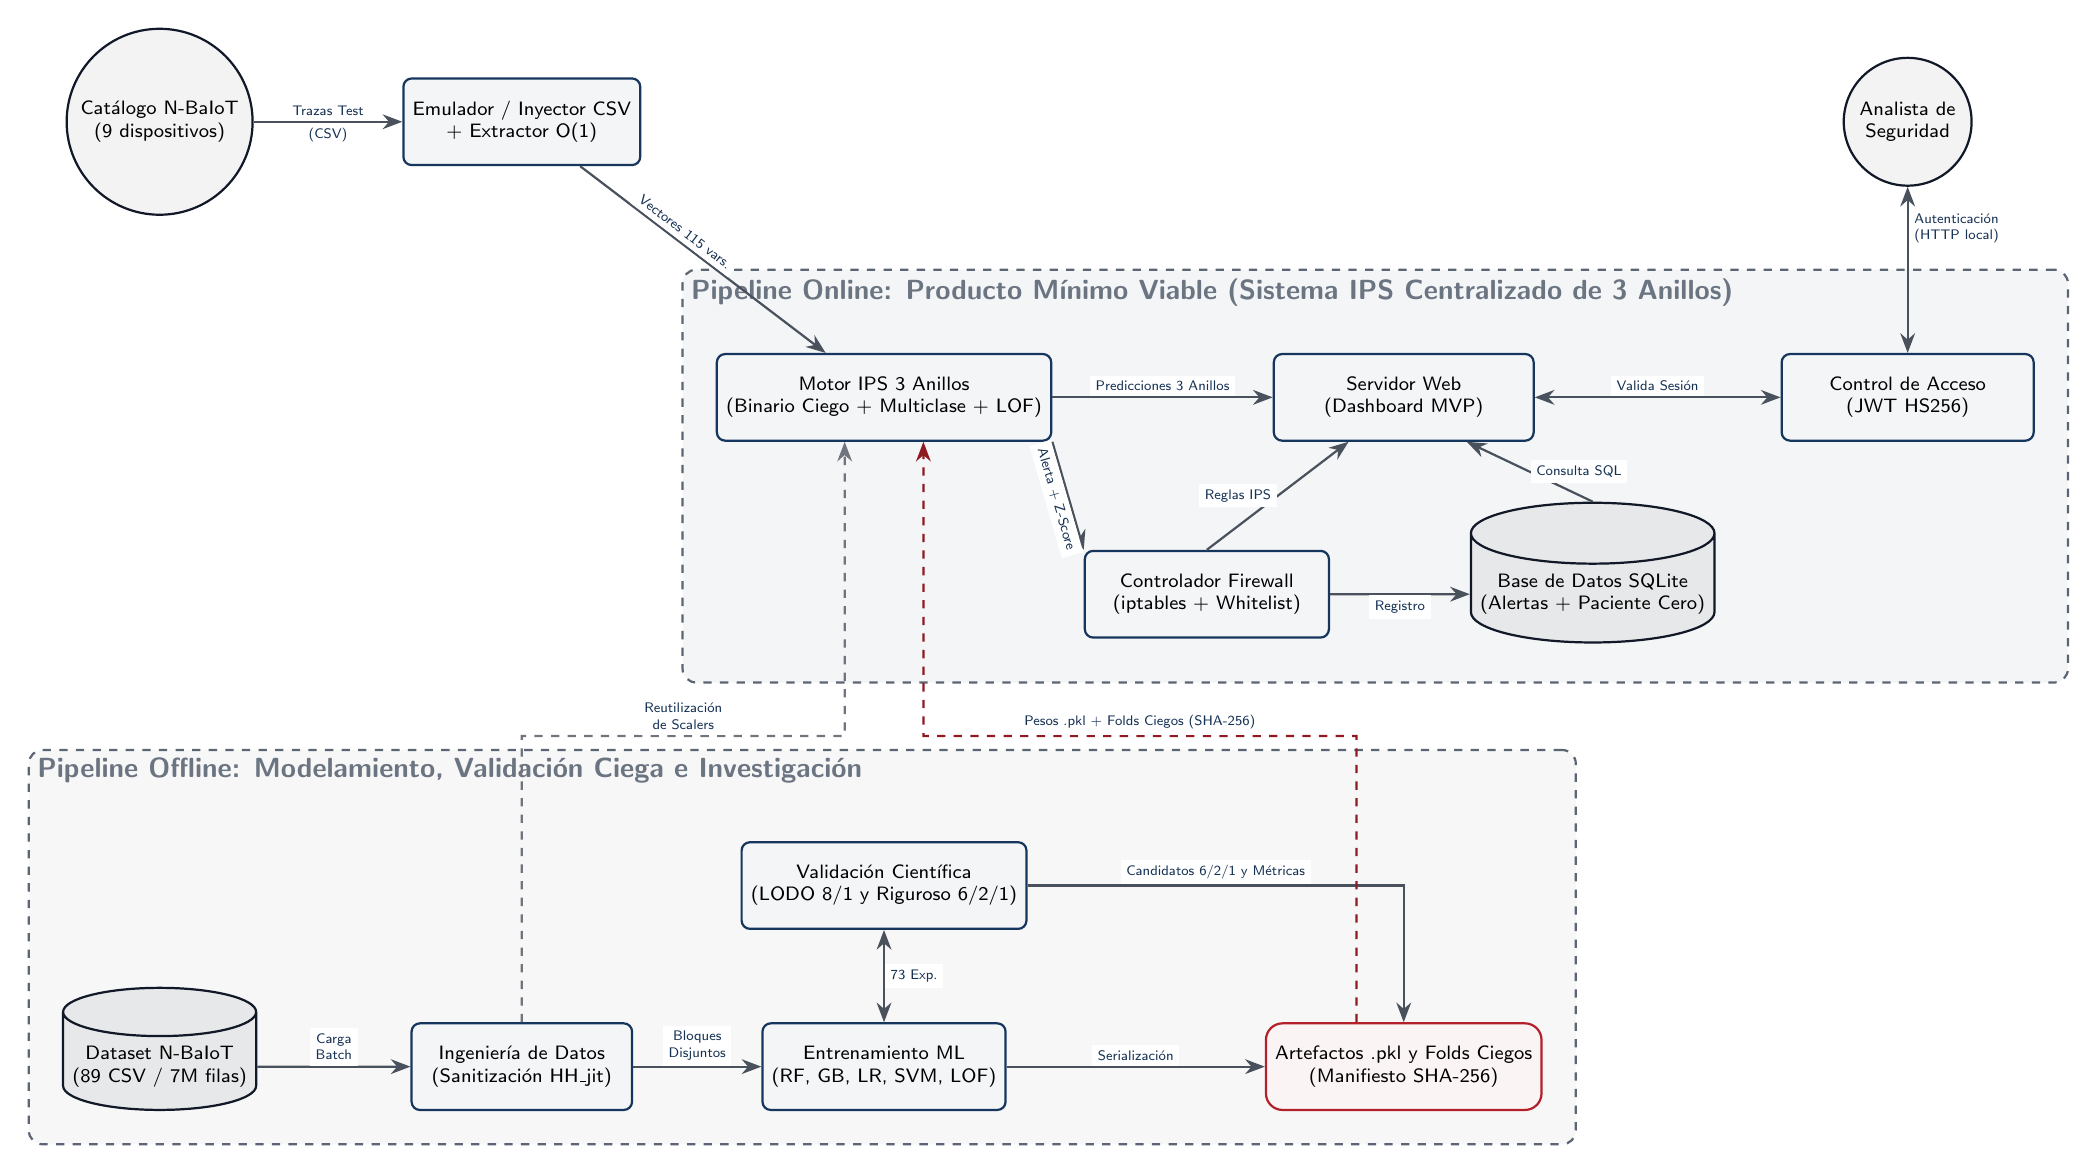
\begin{tikzpicture}[
  actor/.style={circle, draw=CINFNavy, fill=CINFNavy!5, thick, minimum size=1.5cm, align=center, font=\scriptsize\sffamily},
  sysbox/.style={rectangle, draw=CINFBlue, fill=CINFBlue!5, thick, minimum width=2.8cm, minimum height=1.1cm, align=center, font=\scriptsize\sffamily, rounded corners=3pt},
  db/.style={cylinder, draw=CINFNavy, fill=CINFNavy!10, thick, minimum width=2cm, minimum height=1.1cm, align=center, font=\scriptsize\sffamily, shape border rotate=90, aspect=0.25},
  modelbox/.style={rectangle, draw=CINFRed, fill=CINFRed!5, thick, minimum width=2.8cm, minimum height=1.1cm, align=center, font=\scriptsize\sffamily, rounded corners=6pt},
  arr/.style={-{Stealth[length=2.5mm]}, thick, CINFGray!80!black},
  biarr/.style={{Stealth[length=2.5mm]}-{Stealth[length=2.5mm]}, thick, CINFGray!80!black},
  lbl/.style={font=\tiny\sffamily, text=CINFBlue!90!black, fill=white, inner sep=2pt, align=center},
  groupbox/.style={rectangle, draw=CINFGray, thick, dashed, inner sep=12pt, rounded corners=5pt},
  grouplabel/.style={font=\sffamily\bfseries, text=CINFGray!90, anchor=north west}
]

% 1. EXTERNAL ACTORS (Top layer, y=3.5)
\node[actor]    (iot)         at (0, 3.5) {Catálogo N-BaIoT\\(9 dispositivos)};
\node[sysbox]   (emulator)    at (4.6, 3.5) {Emulador / Inyector CSV\\+ Extractor O(1)};
\node[actor]    (admin)       at (22.2, 3.5) {Analista de\\Seguridad};

% 2. ONLINE PIPELINE (Middle layer, y=0)
\node[sysbox, minimum width=3.6cm] (inference)   at (9.2, 0) {Motor IPS 3 Anillos\\(Binario Ciego + Multiclase + LOF)};
\node[sysbox, minimum width=3.1cm] (firewall)    at (13.3, -2.5) {Controlador Firewall\\(iptables + Whitelist)};
\node[db]       (db_alerts)   at (18.2, -2.5) {Base de Datos SQLite\\(Alertas + Paciente Cero)};
\node[sysbox, minimum width=3.3cm] (dashboard)   at (15.8, 0) {Servidor Web\\(Dashboard MVP)};
\node[sysbox, minimum width=3.2cm] (auth)        at (22.2, 0) {Control de Acceso\\(JWT HS256)};

% Online Connections
\draw[arr] (iot) -- (emulator) node[midway, lbl, above] {Trazas Test} node[midway, lbl, below] {(CSV)};
\draw[arr] (emulator) -- (inference) node[pos=0.40, lbl, above, sloped] {Vectores 115 vars.};
\draw[arr] (inference.south east) -- (firewall.north west) node[midway, lbl, below, sloped] {Alerta + Z-Score};
\draw[arr] (firewall.north) -- ([xshift=-0.7cm]dashboard.south) node[midway, lbl, left] {Reglas IPS};
\draw[arr] (firewall) -- (db_alerts) node[midway, lbl, below] {Registro};
\draw[arr] (inference.east) -- (dashboard.west) node[midway, lbl, above] {Predicciones 3 Anillos};
\draw[arr] (db_alerts.north) -- ([xshift=0.8cm]dashboard.south) node[midway, lbl, right] {Consulta SQL};
\draw[biarr] (dashboard) -- (auth) node[midway, lbl, above] {Valida Sesión};
\draw[biarr] (auth) -- (admin) node[pos=0.75, lbl, right] {Autenticación\\(HTTP local)};

\begin{scope}[on background layer]
  \coordinate (online_top) at (9.2, 1.2);
  \coordinate (online_bottom) at (9.2, -3.2);
  \node[groupbox, fill=CINFBlue!5, fit=(inference) (firewall) (db_alerts) (dashboard) (auth) (online_top) (online_bottom)] (online) {};
  \node[grouplabel] at (online.north west) {Pipeline Online: Producto Mínimo Viable (Sistema IPS Centralizado de 3 Anillos)};
\end{scope}

% 3. OFFLINE PIPELINE (Bottom layer, y=-8.5)
\node[db]       (dataset)     at (0, -8.5) {Dataset N-BaIoT\\(89 CSV / 7M filas)};
\node[sysbox]   (preproc_off) at (4.6, -8.5) {Ingeniería de Datos\\(Sanitización HH\_jit)};
\node[sysbox]   (train)       at (9.2, -8.5) {Entrenamiento ML\\(RF, GB, LR, SVM, LOF)};
\node[sysbox]   (eval)        at (9.2, -6.2) {Validación Científica\\(LODO 8/1 y Riguroso 6/2/1)};
\node[modelbox, minimum width=3.5cm] (registry) at (15.8, -8.5) { Artefactos .pkl y Folds Ciegos\\(Manifiesto SHA-256)};

% Offline Connections
\draw[arr] (dataset) -- (preproc_off) node[midway, lbl, above] {Carga\\Batch};
\draw[arr] (preproc_off) -- (train) node[midway, lbl, above] {Bloques\\Disjuntos};
\draw[biarr] (train) -- (eval) node[midway, lbl, right] {73 Exp.};
\draw[arr] (train) -- (registry) node[midway, lbl, above] {Serialización};
\draw[arr] (eval.east) -| (registry.north) node[pos=0.25, lbl, above] {Candidatos 6/2/1 y Métricas};

\begin{scope}[on background layer]
  \coordinate (offline_top) at (9.2, -4.9);
  \node[groupbox, fill=CINFGray!5, fit=(dataset) (preproc_off) (train) (eval) (registry) (offline_top)] (offline) {};
  \node[grouplabel] at (offline.north west) {Pipeline Offline: Modelamiento, Validación Ciega e Investigación};
\end{scope}

% 4. CROSS CONNECTIONS (From Offline UP to Online)
\draw[arr, dashed, CINFRed!80!black] ([xshift=-0.6cm]registry.north) -- (15.2, -4.3) -- (9.7, -4.3) node[midway, lbl, above] {Pesos .pkl + Folds Ciegos (SHA-256)} -- ([xshift=0.5cm]inference.south);
\draw[arr, dashed, CINFNavy!60] (preproc_off.north) -- (4.6, -4.3) -- (8.7, -4.3) node[midway, lbl, above] {Reutilización\\de Scalers} -- ([xshift=-0.5cm]inference.south);
\end{tikzpicture}
}%
\caption{Arquitectura general del sistema de doble pipeline: monitoreo e inferencia en 3 anillos con enrutamiento ciego 6/2/1, detección de paciente cero y generación de reglas de cortafuegos en la parte superior (Pipeline Online), alimentado por el pipeline de ingeniería de datos, validación científica y artefactos verificados con SHA-256 en la parte inferior (Pipeline Offline).}
\label{fig:arquitectura}
\end{figure}

\textbf{Estado de implementación:} la consola procesa vectores ya extraídos del catálogo y registra alertas en SQLite dentro de la aplicación Streamlit. Su autenticación usa credenciales configurables y JWT local con expiración; no existe un API Gateway independiente ni se acreditó HTTPS productivo. El extractor desde cabeceras es experimental y no implementa captura. Los candidatos del protocolo revisado se guardan en un directorio separado verificados mediante manifiesto \texttt{SHA-256} y pueden activarse opcionalmente en la consola mediante el modo de enrutamiento ciego 6/2/1 por dispositivo, conservando separados los modelos históricos de línea base. La generación de comandos de firewall y el estado de cuarentena son demostraciones sin ejecución ni verificación de reglas reales.

\subsection{Modelamiento de datos}
El dataset N-BaIoT contiene tráfico de red capturado desde nueve dispositivos IoT comerciales, organizado en archivos CSV independientes por dispositivo y por tipo de tráfico (benigno o de ataque). La Tabla~\ref{tab:dispositivos} lista los dispositivos incluidos.

\begin{table}[H]
\centering
\caption{Dispositivos IoT incluidos en el dataset N-BaIoT.}
\label{tab:dispositivos}
\small
\begin{tabularx}{\textwidth}{c l X}
\toprule
\textbf{\#} & \textbf{Dispositivo} & \textbf{Categoría} \\
\midrule
1 & Danmini Doorbell & Timbre inteligente \\
2 & Ecobee Thermostat & Termostato \\
3 & Ennio Doorbell & Timbre inteligente \\
4 & Philips B120N/10 Baby Monitor & Monitor de bebé \\
5 & Provision PT-737E Security Camera & Cámara de seguridad \\
6 & Provision PT-838 Security Camera & Cámara de seguridad \\
7 & Samsung SNH 1011 Webcam & Cámara web \\
8 & SimpleHome XCS7-1002-WHT & Cámara de seguridad \\
9 & SimpleHome XCS7-1003-WHT & Cámara de seguridad \\
\bottomrule
\end{tabularx}
\end{table}

\subsubsection{Estructura de las características}
Cada muestra del dataset contiene 115 características numéricas extraídas a partir de metadatos del tráfico de red, calculadas sobre ventanas temporales de distinto tamaño. Las características se agrupan en cinco familias, descritas en la Tabla~\ref{tab:features}.

\begin{table}[H]
\centering
\caption{Familias de características del dataset N-BaIoT.}
\label{tab:features}
\small
\begin{tabularx}{\textwidth}{p{2.0cm} p{3.8cm} X}
\toprule
\textbf{Familia} & \textbf{Alcance} & \textbf{Descripción} \\
\midrule
MI & Canal de comunicación & Estadísticas agregadas sobre el comportamiento del canal (tamaño, conteo). \\
H & IP de origen (\textit{host}) & Estadísticas del tráfico saliente desde una IP de origen específica. \\
HH & Par origen-destino & Estadísticas del tráfico entre un par de direcciones IP. \\
HpHp & Par origen-destino con puertos & Igual que HH pero diferenciando además por puerto de origen y destino. \\
HH\_jit & Par origen-destino (\textit{jitter}) & Variabilidad temporal (\textit{jitter}) del tráfico entre un par de IPs. \\
\bottomrule
\end{tabularx}
\end{table}

Dentro de cada familia, las estadísticas se calculan sobre estadísticas con cinco tasas de decaimiento $\lambda \in \{5,3,1,0{,}1,0{,}01\}$, con semividas de $0{,}2$, $1/3$, $1$, $10$ y $100$ segundos, respectivamente; no son ventanas rectangulares, y para cada ventana se extraen métricas como peso (número de paquetes), media, desviación estándar, magnitud, radio y covarianza del tamaño de los paquetes. Esto genera el total de 115 columnas numéricas por muestra.

\subsubsection{Variable objetivo y codificación de clases}
El dataset original no incluye una columna de etiqueta explícita; la clase se infiere a partir del archivo de origen de cada muestra:
\begin{itemize}
  \item \textbf{Clase 0 --- Benigno:} tráfico capturado durante la operación normal del dispositivo.
  \item \textbf{Clase 1 --- Malicioso:} tráfico generado tras la infección con Mirai o BASHLITE. Incluye subtipos de ataque (ACK flood, SYN flood, UDP flood, escaneo de puertos, entre otros).
\end{itemize}

Para el entrenamiento se utilizará una clasificación binaria (benigno vs.\ malicioso). La información del subtipo de ataque se conservará como metadato para análisis posteriores, pero no se usará como variable objetivo.

\subsubsection{Flujo de transformación de datos}
La Figura~\ref{fig:flujo-datos} presenta el flujo de transformación desde los archivos CSV crudos hasta los tensores listos para modelamiento, separando particiones antes del ajuste estadístico. Esto reduce riesgos de fuga, pero no certifica independencia entre vectores ni capturas.

\begin{figure}[H]
\centering
\resizebox{0.96\textwidth}{!}{%
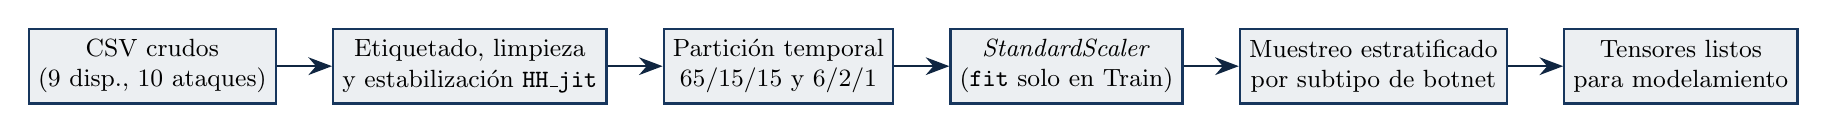
\begin{tikzpicture}[
  block/.style={rectangle, draw=CINFBlue, fill=CINFBlue!8, thick, minimum height=0.95cm, minimum width=2.2cm, align=center, font=\small},
  arr/.style={-{Stealth[length=3mm]}, thick, CINFBlue!70!black}
]
\node[block] (raw) {CSV crudos\\(9 disp., 10 ataques)};
\node[block, right=0.7cm of raw] (clean) {Etiquetado, limpieza\\y estabilización \texttt{HH\_jit}};
\node[block, right=0.7cm of clean] (split) {Partición temporal\\65/15/15 y 6/2/1};
\node[block, right=0.7cm of split] (norm) {\textit{StandardScaler}\\(\texttt{fit} solo en Train)};
\node[block, right=0.7cm of norm] (balance) {Muestreo estratificado\\por subtipo de botnet};
\node[block, right=0.7cm of balance] (ready) {Tensores listos\\para modelamiento};
\draw[arr] (raw) -- (clean);
\draw[arr] (clean) -- (split);
\draw[arr] (split) -- (norm);
\draw[arr] (norm) -- (balance);
\draw[arr] (balance) -- (ready);
\end{tikzpicture}
}%
\caption{Flujo de transformación de datos del preprocesamiento con separación de roles estadísticos.}
\label{fig:flujo-datos}
\end{figure}

\subsection{Diseño experimental}
El protocolo vigente es el descrito en la metodología y resumido en la Figura~\ref{fig:diseno-exp}. Cada experimento conserva la configuración, el umbral, las predicciones, la procedencia archivo/fila y la matriz de confusión. Se completaron 3 experimentos temporales, 27 por dispositivo, 16 de familia excluida y 27 ablaciones adicionales: 73 en total. Los resultados actuales se consideran evidencia de desarrollo; un test final futuro debe reservar capturas independientes.

\begin{figure}[H]
\centering
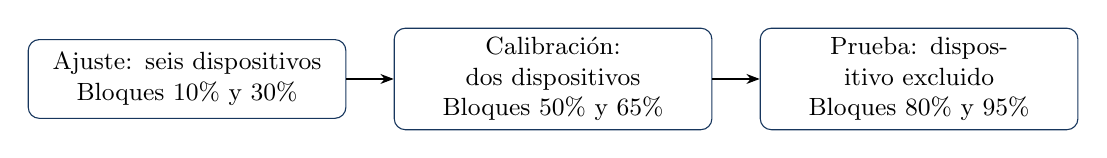
\begin{tikzpicture}[node distance=0.6cm, every node/.style={draw=CINFBlue,rounded corners,align=center,font=\small,text width=3.8cm,minimum height=1cm}]
\node (a) {Ajuste: seis dispositivos\\Bloques 10\% y 30\%};
\node[right=of a] (b) {Calibración: dos dispositivos\\Bloques 50\% y 65\%};
\node[right=of b] (c) {Prueba: dispositivo excluido\\Bloques 80\% y 95\%};
\draw[-{Stealth}] (a)--(b);\draw[-{Stealth}] (b)--(c);
\end{tikzpicture}
\caption{Roles separados en el protocolo revisado. Se rota el dispositivo de prueba. La exclusión de una familia se aplica también a calibración.}
\label{fig:diseno-exp}
\end{figure}

\subsection{Selección y justificación de algoritmos}
Los cuatro algoritmos seleccionados corresponden a técnicas de clasificación supervisada ampliamente validadas en la literatura de detección de intrusiones. La selección prioriza modelos de Machine Learning clásico por sobre Deep Learning, en coherencia con el objetivo del proyecto de lograr un desempeño competitivo con un costo computacional significativamente menor. La Tabla~\ref{tab:algoritmos} resume las características relevantes de cada modelo.

\begin{table}[H]
\centering
\caption{Algoritmos seleccionados: características y justificación.}
\label{tab:algoritmos}
\small
\begin{tabularx}{\textwidth}{p{2.5cm} p{2.5cm} p{2.8cm} X}
\toprule
\textbf{Algoritmo} & \textbf{Complejidad de entrenamiento} & \textbf{Complejidad de inferencia} & \textbf{Justificación} \\
\midrule
Regresión Logística & $O(n \cdot d)$ & $O(d)$ & Línea base simple y rápida; permite evaluar si modelos más complejos aportan mejora real. \\
Random Forest & $O(k \cdot n \cdot d \cdot \log n)$ & $O(k \cdot \text{prof.})$ & Robusto frente a \textit{overfitting}; entrega \textit{feature importance} nativamente; adecuado para datos tabulares. \\
Support Vector Machine & $O(n \cdot d)$ (formulación primal \texttt{LinearSVC}) & $O(d)$ & Hiperplano de margen máximo en espacio de 115 dimensiones con calibración sigmoide de Platt; contraste frente a métodos basados en árboles. \\
Gradient Boosting & $O(k \cdot n \cdot d)$ & $O(k \cdot \text{prof.})$ & Estado del arte en datos tabulares (\texttt{HistGradientBoosting}); alta precisión y baja tasa de falsos positivos en dispositivos no vistos. \\
\bottomrule
\end{tabularx}
\end{table}

\noindent Donde $n$ es el número de muestras, $d$ el número de características, $k$ el número de árboles (en Random Forest y Gradient Boosting), y \textit{prof.} la profundidad promedio de los árboles.

\textbf{¿Por qué no Deep Learning?} La decisión de priorizar Machine Learning clásico se fundamenta en tres argumentos:
\begin{enumerate}
  \item \textbf{Costo computacional:} los modelos de Deep Learning (autoencoders, CNN-BiLSTM) pueden requerir mayor capacidad computacional según su configuración; no se midió aquí una comparación controlada de recursos, mientras que los modelos seleccionados se entrenan en segundos sobre CPU convencional.
  \item \textbf{Explicabilidad:} Random Forest y Gradient Boosting permiten extraer la importancia relativa de cada característica (\textit{feature importance}), lo que posibilita explicar al analista \textit{por qué} el sistema clasificó un tráfico como malicioso. La importancia global tampoco explica por sí sola cada predicción ni prueba causalidad.
  \item \textbf{Viabilidad de despliegue:} el escenario objetivo es un dispositivo de borde (\textit{edge}) o un computador doméstico con recursos limitados. Un modelo de Random Forest o Gradient Boosting serializado ocupa entre 0,3~MB y 2,5~MB; una red neuronal profunda requiere decenas de megabytes y dependencias pesadas.
\end{enumerate}

\subsection{\textit{Stack} tecnológico}
La Tabla~\ref{tab:stack} presenta las herramientas y librerías seleccionadas, junto con la justificación de cada elección. Todas las herramientas son de código abierto y gratuitas, en coherencia con la restricción de presupuesto cero del proyecto.

\begin{table}[H]
\centering
\caption{\textit{Stack} tecnológico del proyecto.}
\label{tab:stack}
\small
\begin{tabularx}{\textwidth}{p{2.5cm} p{2.2cm} X}
\toprule
\textbf{Herramienta} & \textbf{Versión} & \textbf{Rol y justificación} \\
\midrule
Python & 3.13 & Lenguaje principal; ecosistema dominante en ML y ciencia de datos. \\
scikit-learn & $\geq$ 1.5 & Implementación de referencia de los algoritmos, validación cruzada y calibración probabilística. \\
pandas / NumPy & $\geq$ 2.0 / 1.26 & Ingesta tabular vectorizada, partición temporal y álgebra lineal eficiente. \\
SciPy & $\geq$ 1.13 & Pruebas de significancia estadística no paramétrica (rangos con signo de Wilcoxon). \\
Streamlit & $\geq$ 1.30 & Framework para el dashboard web del MVP con caché de recursos en memoria (\texttt{@st.cache\_resource}). \\
SQLite3 & Nativo & Base de datos relacional transaccional para persistencia histórica de incidentes con consultas parametrizadas. \\
joblib / hashlib & $\geq$ 1.3 & Serialización de artefactos \texttt{.pkl} acompañada de verificación de integridad criptográfica \texttt{SHA-256}. \\
unittest & Nativo & Suite de pruebas automatizadas de regresión, latencia, no-fuga temporal y seguridad. \\
\bottomrule
\end{tabularx}
\end{table}

El entorno de software y las configuraciones experimentales se registran junto con los resultados para facilitar su reproducción.

% -----------------------------------------------------------------------------
\section{Implementación y producto mínimo viable}
\subsection{Estructura modular y recorrido funcional}
El directorio \texttt{proyecto-iot-ml} contiene módulos de datos, modelos, reproducción y persistencia, además de la interfaz Streamlit. \texttt{src/models/rigorous.py} implementa el protocolo revisado; \texttt{src/models/reporting.py} distingue métricas históricas, adaptativas y multiclase sin copiar resultados no evaluados. Los candidatos nuevos conservan modelo, columnas, umbral y metadatos en cada experimento. El repositorio remoto identifica el proyecto, pero la publicación de los cambios locales debe verificarse para garantizar reproducibilidad.

El recorrido demostrado comprende autenticación, carga de modelos con comprobación SHA-256, selección de una traza de ataque y otra benigna, inferencia y persistencia de alertas. La reproducción continua queda bajo control del analista. Las direcciones y dispositivos del catálogo no son un descubrimiento de la red del usuario.

\subsection{Controles y limitaciones funcionales}
Las consultas SQLite son parametrizadas. Los hashes permiten comprobar consistencia con el manifiesto local; no prueban autenticidad si se sustituye también ese manifiesto. Las credenciales de ejemplo deben sustituirse antes de distribuir el sistema. La importancia global y las desviaciones estandarizadas son ayudas exploratorias y no causas físicas demostradas. El primer incidente guardado identifica la primera alerta observada y no un paciente cero causal.

La cuarentena de la interfaz actualiza el estado de sesión y genera comandos de mitigación (\texttt{iptables}, \texttt{nftables} y \texttt{conntrack}) con lista blanca anti-bloqueo (\textit{Anti-Lockout}), sin ejecutar bloqueos reales en el router anfitrión. La interfaz incorpora avisos explícitos diferenciando la reproducción controlada del catálogo respecto de una captura productiva, y activa por defecto el enrutamiento ciego 6/2/1 (\texttt{device\_1\_rf} a \texttt{device\_9\_rf}). El extractor online requiere validación numérica y control de memoria antes de un despliegue físico. El MVP no acredita operación autónoma, descubrimiento de activos ni eficacia productiva.

\subsection{Decisiones y pruebas de avance}
Se mantienen artefactos históricos para reproducibilidad; se evita promover candidatos usando el test; se conserva el dashboard como consola del analista con tres anillos de defensa (Anillo~1 binario ciego 6/2/1, Anillo~2 multiclase de 10 subtipos de botnet y Anillo~3 no supervisado \texttt{LocalOutlierFactor}) y se difieren las pruebas físicas. La sanitización neutraliza diez columnas de media/varianza de jitter, preservando sus pesos; no aplica la transformación logarítmica descrita en versiones anteriores. En el nuevo protocolo se excluyen esas diez columnas constantes.

La suite contiene 25 pruebas en cuatro módulos: contratos del pipeline, particiones y calibración, integridad del reporte, e incorporación dinámica de nuevos equipos (\texttt{tests/test\_onboarding.py}). Además, la interfaz se rediseñó bajo una arquitectura minimalista en cinco pestañas con escenarios guiados de un clic, protección contra fuerza bruta en el inicio de sesión (\textit{rate limiting}), traductor de desviaciones Z-Score a lenguaje no técnico, exportación forense CSV y un módulo de \textbf{incorporación dinámica (\texttt{device\_onboarding.py})} que implementa un \textit{Modo Aprendizaje 24h} (auto-calibración $\tau_{\text{personal}} = \min(0{,}95,\max(0{,}50, Q_{99{,}5}+0{,}05))$ sin bloqueo prematuro) y un \textit{Modo Observación Social} ante ráfagas de invitados ($\ge 3$ equipos nuevos simultáneos). Las pruebas del generador de comandos verifican texto y protección de lista blanca, no eficacia de aislamiento físico. La comprobación del extractor no establece equivalencia matemática con el extractor de referencia Kitsune. La Figura~\ref{fig:mvp} ilustra la interfaz operativa del prototipo durante una comprobación local.

\begin{figure}[H]
\centering
\IfFileExists{dashboard_funcionando.png}{%
  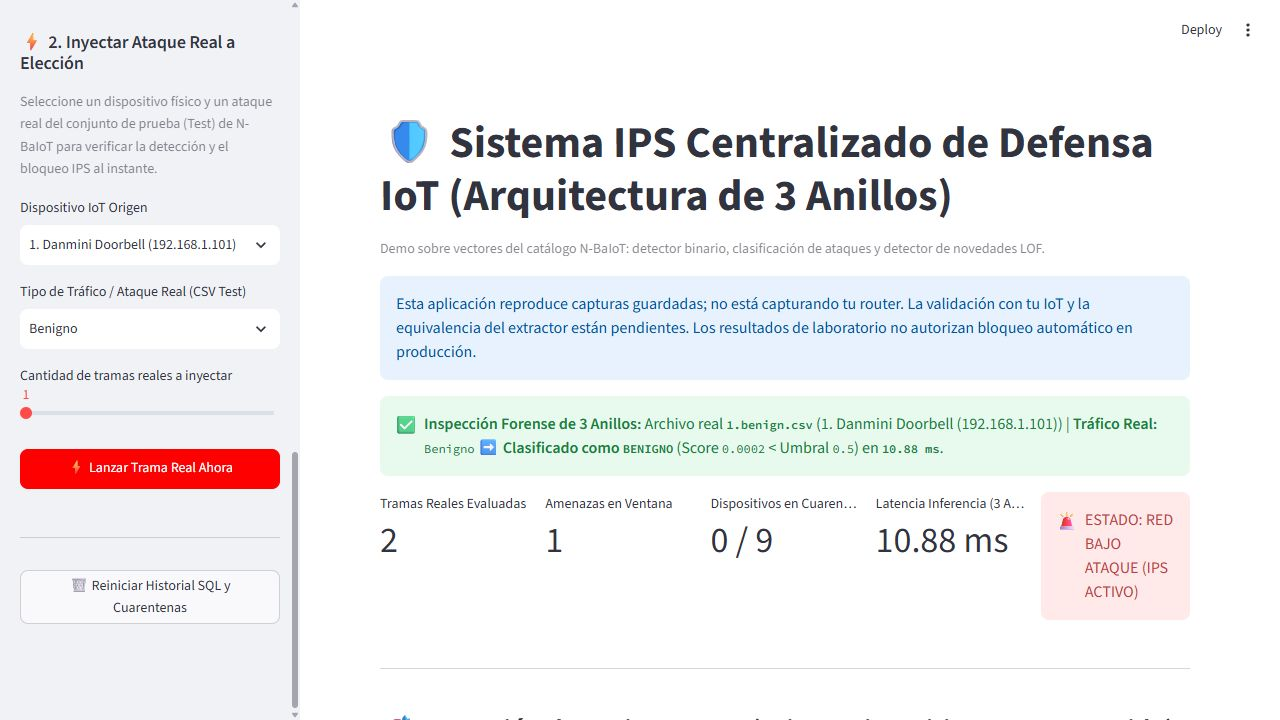
\includegraphics[width=\textwidth]{dashboard_funcionando.png}%
}{%
  \IfFileExists{dashboard_funcionando.jpg}{%
    \includegraphics[width=\textwidth]{dashboard_funcionando.jpg}%
  }{%
    \fbox{\parbox[c][4cm][c]{0.8\textwidth}{\centering Consola Streamlit MVP (\texttt{http://localhost:8501})}}%
  }%
}
\caption{Evidencia local de la consola MVP durante la comprobación funcional en \texttt{localhost:8501}. Los indicadores corresponden a reproducción controlada del catálogo N-BaIoT; los comandos de cuarentena son demostrativos y no aplican bloqueo real sobre el router.}
\label{fig:mvp}
\end{figure}

\subsection{Responsabilidades de los componentes y evidencias}
La Tabla~\ref{tab:modulos} detalla la implementación para permitir relacionar arquitectura, código y pruebas. El flujo de datos y los diagramas anteriores se complementan con esta vista del repositorio.
\begin{longtable}{p{0.30\textwidth}p{0.61\textwidth}}
\caption{Componentes implementados y evidencia verificable.}\label{tab:modulos}\\
\toprule
\textbf{Componente} & \textbf{Responsabilidad y límite}\\
\midrule
\endfirsthead
\toprule
\textbf{Componente} & \textbf{Responsabilidad y límite}\\
\midrule
\endhead
\texttt{src/data/preprocess.py} & Carga el catálogo, deriva etiquetas del archivo, excluye metadatos de las entradas y prepara las particiones históricas. Neutraliza diez columnas de media/varianza de jitter; no aplica una transformación logarítmica.\\
\addlinespace
\texttt{src/models/baseline.py} & Reproduce los clasificadores y protocolos históricos. Conserva CV y LODO como antecedentes con las limitaciones metodológicas declaradas.\\
\addlinespace
\texttt{src/models/rigorous.py} & Inspecciona datos, selecciona bloques, separa roles de dispositivos, calibra umbrales y ejecuta exclusiones y ablaciones. Guarda procedencia, configuración, predicciones y candidatos separados.\\
\addlinespace
\texttt{src/models/reporting.py} & Presenta tareas y métricas diferenciadas. No asigna al modelo adaptativo resultados que no fueron evaluados; distingue clasificación multiclase original y agrupada.\\
\addlinespace
\texttt{src/streaming/emulator.py} & Reproduce vectores del catálogo de prueba. No recibe paquetes de una interfaz de red. Sus fallbacks sintéticos requieren tratamiento explícito si falta el catálogo.\\
\addlinespace
\texttt{incident\_store.py} & Persiste y consulta alertas mediante SQLite y parámetros SQL. La primera alerta guardada no acredita el origen causal de una infección.\\
\addlinespace
\texttt{live\_feature\_extractor.py} & Prototipo incremental desde cabeceras. La dimensión de salida no acredita equivalencia matemática con N-BaIoT; covarianza y gestión de estado requieren validación.\\
\addlinespace
\texttt{firewall\_controller.py} & Genera propuestas de comandos y aplica una lista blanca estática al generador. No ejecuta ni confirma políticas en un router.\\
\addlinespace
\texttt{device\_onboarding.py} & Gestiona incorporación dinámica de equipos nuevos: \textit{Modo Aprendizaje 24h} (\textit{fail-open} con auto-calibración $Q_{99{,}5}+0{,}05$) y \textit{Modo Observación Social} ante ráfagas de invitados ($\ge 3$ equipos) para evitar falsas alarmas masivas. En el MVP opera sobre simulación acelerada.\\
\addlinespace
\texttt{app/app.py} & Consola minimalista en cinco pestañas con autenticación JWT (\textit{rate limiting}), verificación \texttt{SHA-256}, escenarios guiados de un clic, inferencia ciega 6/2/1, traductor humano de Z-Score, exportación CSV y simulación de nuevos equipos/invitados. No constituye un servicio autónomo de captura.\\
\addlinespace
\texttt{tests/} & Veinticinco pruebas en cuatro módulos (\texttt{test\_pipeline.py}, \texttt{test\_rigorous.py}, \texttt{test\_reporting.py} y \texttt{test\_onboarding.py}). No sustituyen evaluación de carga o pruebas físicas en router.\\
\bottomrule
\end{longtable}

\subsection{Registro de decisiones técnicas actualizado}
La Tabla~\ref{tab:decisiones-tecnicas} conserva la trazabilidad de decisiones, alternativas y restricciones. Las decisiones vinculan los requisitos con la implementación y sus limitaciones.
\begin{longtable}{p{0.16\textwidth}p{0.36\textwidth}p{0.36\textwidth}}
\caption{Decisiones arquitectónicas y metodológicas del proyecto.}\label{tab:decisiones-tecnicas}\\
\toprule
\textbf{Decisión} & \textbf{Justificación y alternativa} & \textbf{Evidencia y restricción}\\
\midrule
\endfirsthead
\toprule
\textbf{Decisión} & \textbf{Justificación y alternativa} & \textbf{Evidencia y restricción}\\
\midrule
\endhead
ADR-01: artefactos separados & Cargar modelos persistidos evita entrenar al iniciar la interfaz. Se descarta el reentrenamiento implícito en cada sesión. & Registro histórico y candidatos de experimentos en carpetas distintas. La promoción requiere evaluación explícita.\\
\addlinespace
ADR-02: roles separados & Separar dispositivos de ajuste, calibración y prueba reduce contaminación del umbral. La CV histórica se conserva como antecedente. & Protocolo seis/dos/uno y pruebas de disyunción; dependencia entre capturas todavía posible.\\
\addlinespace
ADR-03: jitter & Neutralizar media/varianza evita depender de determinadas magnitudes de inicialización; preservar pesos mantiene información de actividad. & Diez columnas excluidas en la representación revisada y ablación con valores crudos. No se atribuye mejora causal sin comparación.\\
\addlinespace
ADR-04: observación central & Se proyecta observar desde un punto de red para equipos sin agentes. La alternativa es instrumentar cada dispositivo. & El prototipo utiliza replay CSV. Visibilidad del router, protocolos y captura efectiva pendientes.\\
\addlinespace
ADR-05: acceso y persistencia & JWT local y SQLite permiten demostrar sesión y almacenamiento; las consultas parametrizadas evitan interpolar entradas en SQL. & Login y persistencia probados. Faltan controles productivos de identidades, secretos y sesiones.\\
\addlinespace
ADR-06: integridad & Comparar hashes detecta cambios respecto al manifiesto, frente a cargar artefactos sin comprobarlos. & SHA-256 previo a carga; el manifiesto requiere una procedencia confiable.\\
\addlinespace
ADR-07: aceptación & Reportar fallas de familias excluidas evita seleccionar únicamente escenarios fáciles. & Umbrales fijados antes del test, métricas por escenario y ausencia explícita de aprobación productiva.\\
\bottomrule
\end{longtable}

\subsection{Estado de desarrollo}
Se completaron la auditoría de datos, los 73 experimentos, las pruebas de software y la comprobación del recorrido del prototipo. La validación mediante capturas independientes y la ejecución de políticas en dispositivos físicos permanecen como trabajo futuro.

\section{Evaluación y resultados}

\subsection{Criterios, métricas y protocolo de evaluación}
La evaluación se diseñó bajo los principios de aseguramiento de calidad de CRISP-ML(Q) \cite{studer2021crispmlq}, combinando métricas de clasificación sobre clase maliciosa (precisión, recall, F1-score, FPR, ROC-AUC y precisión media), métricas de eficiencia computacional (latencia unitaria por muestra medida con \texttt{perf\_counter} en CPU) y controles verificables de calidad de software y ciberseguridad (autenticación JWT \texttt{HS256} con \textit{rate limiting}, integridad \texttt{SHA-256}, consultas SQL parametrizadas y 25 pruebas automatizadas).

En la auditoría íntegra del conjunto UCI N-BaIoT se inspeccionaron 7.062.606 filas en 89 archivos CSV (555.932 benignas y 6.506.674 de ataque), verificando cero valores \texttt{NaN} o infinitos. No obstante, la revisión de la partición histórica detectó 1.211 coincidencias exactas sobre 6.785 vectores de prueba tras la sanitización (17,85\%), lo que justificó congelar un protocolo revisado más exigente: seis dispositivos para ajuste (bloques posicionales 10\% y 30\%), dos para calibración de umbral con objetivo empírico $\text{FPR} \le 0{,}1\%$ (bloques 50\% y 65\%) y uno completamente excluido para prueba (bloques 80\% y 95\%), rotando los nueve dispositivos y añadiendo 16 pruebas de exclusión total de familias (\textit{Mirai} vs.\ \textit{BASHLITE}) y 27 ablaciones, totalizando \textbf{73 experimentos reproducibles} (Figura~\ref{fig:protocolo-621}).

\begin{figure}[H]
\centering
\IfFileExists{fig_ppt_protocolo_621.png}{%
  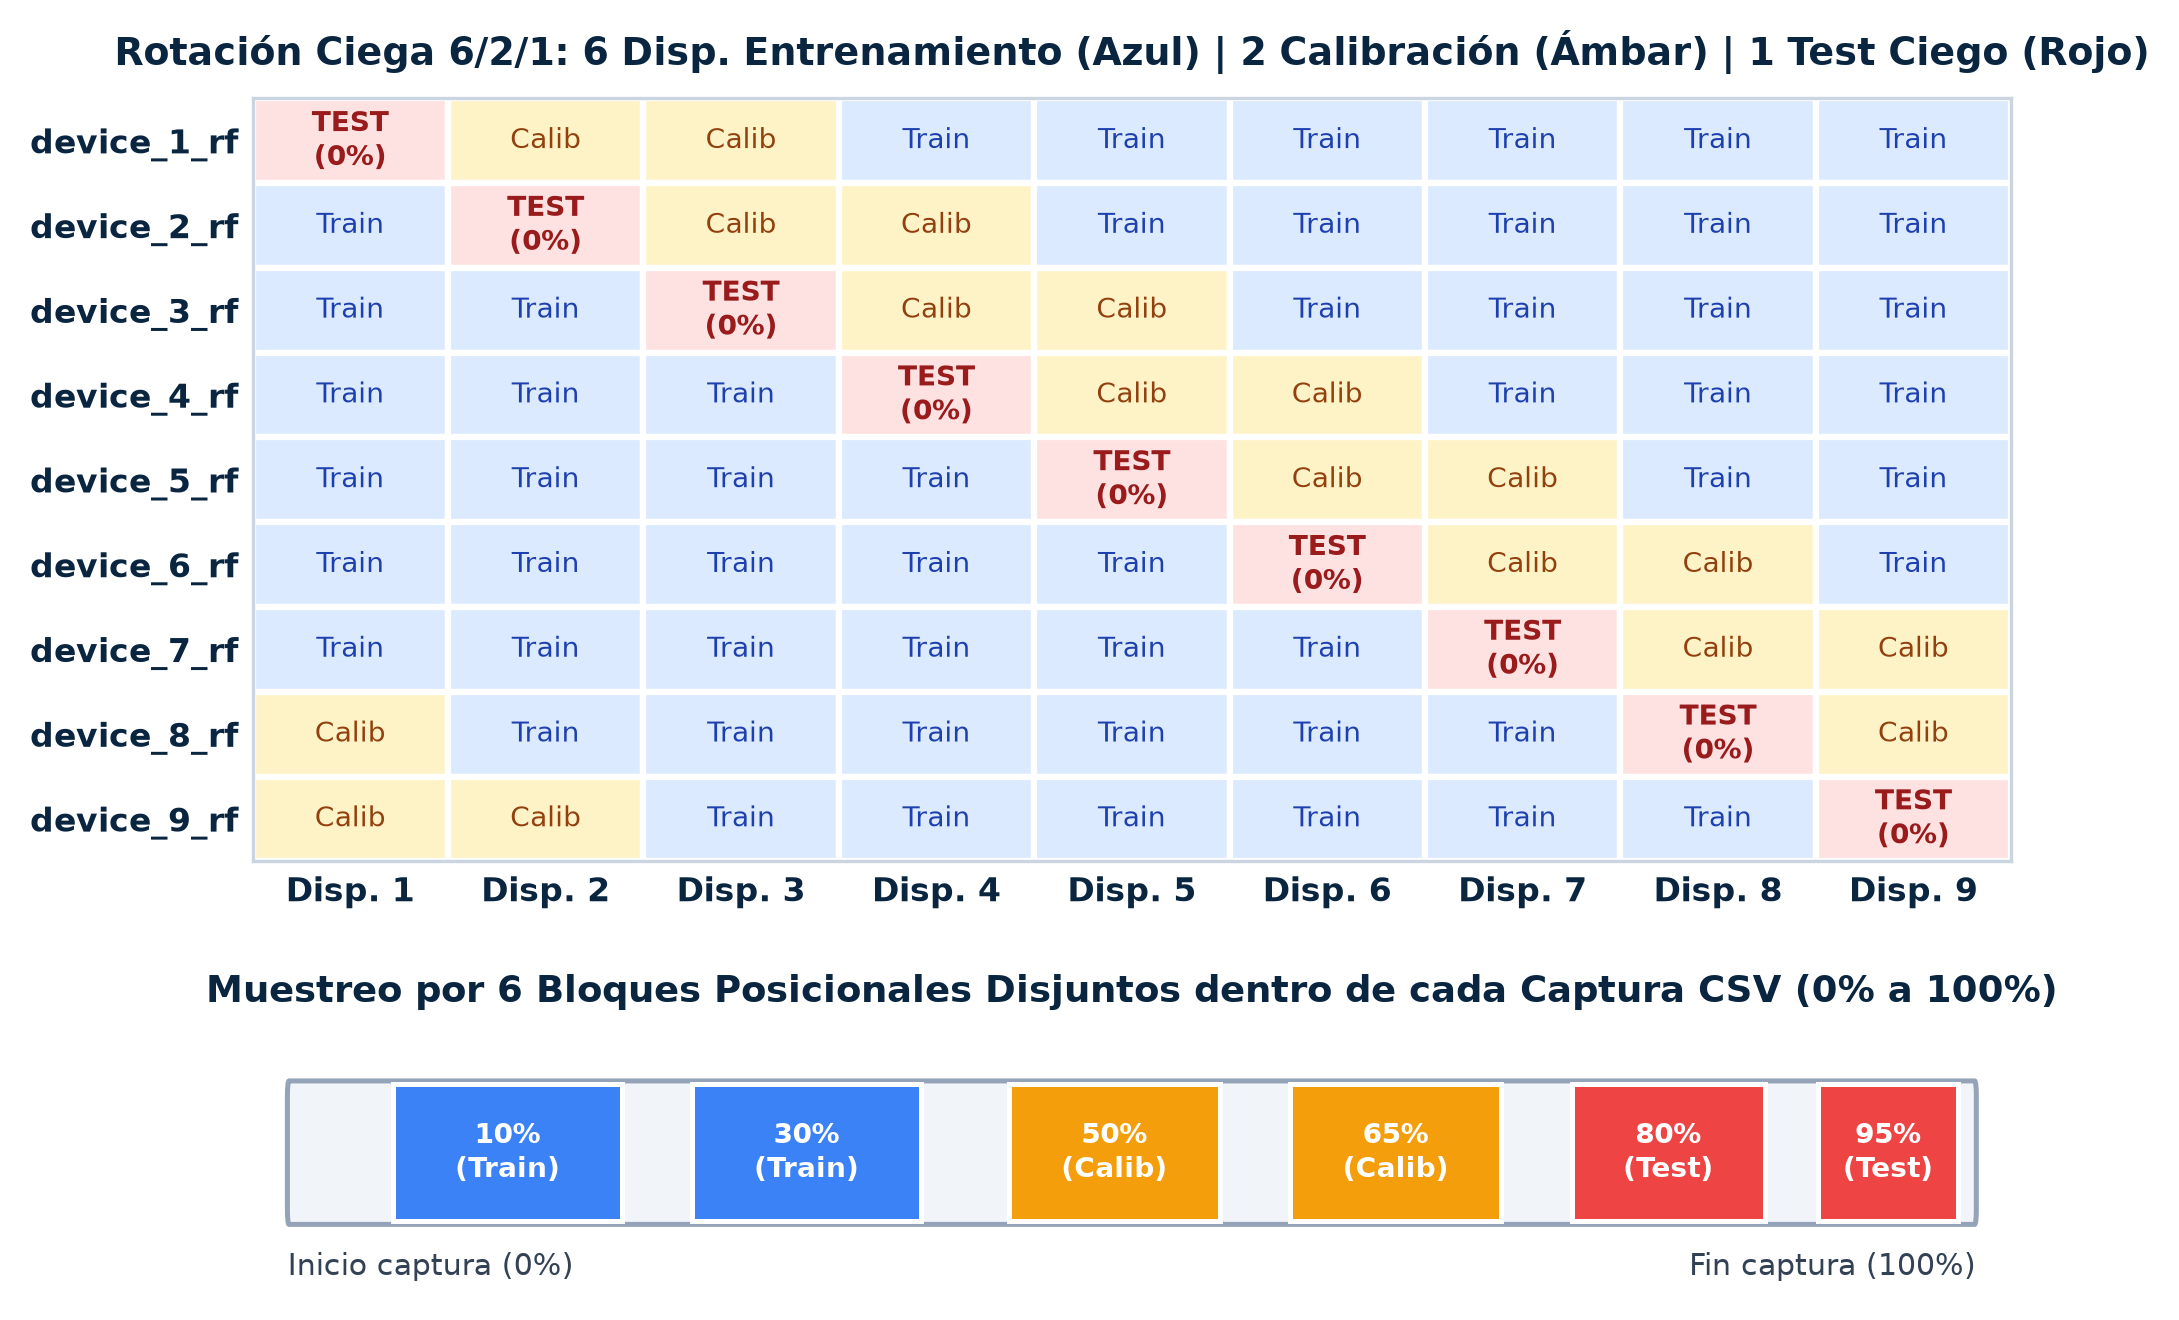
\includegraphics[width=0.92\textwidth]{fig_ppt_protocolo_621.png}%
}{%
  \fbox{\parbox[c][3.5cm][c]{0.8\textwidth}{\centering Matriz de rotación ciega 6/2/1 (9 folds) y 6 bloques posicionales}}%
}
\caption{Matriz de rotación ciega 6/2/1 sobre los nueve dispositivos N-BaIoT (\texttt{device\_1\_rf} a \texttt{device\_9\_rf}) y muestreo por seis bloques posicionales disjuntos dentro de cada archivo CSV.}
\label{fig:protocolo-621}
\end{figure}

\subsection{Resultados técnicos}

\subsubsection{Referencia histórica frente a línea base y arquitectura de tres anillos}
La Tabla~\ref{tab:historico} consolida los resultados de la fase de referencia histórica sobre el conjunto de prueba de 6.785 muestras (3.375 benignas y 3.410 de ataque), contrastando los cinco clasificadores supervisados contra el clasificador trivial (\texttt{DummyClassifier}).

\begin{table}[H]
\centering\footnotesize
\caption{Desempeño histórico de clasificadores supervisados frente a la línea base (prueba interna, $N = 6.785$).}
\label{tab:historico}
\begin{tabularx}{\textwidth}{X c c c c c c}
\toprule
\textbf{Modelo} & \textbf{Exactitud} & \textbf{Precisión} & \textbf{Recall} & \textbf{F1-Score} & \textbf{FPR} & \textbf{Latencia CPU (ms)} \\
\midrule
Clasificador trivial (\texttt{Dummy}) & 49,74\% & 0,0000 & 0,0000 & 0,0000 & 0,00\% & 0,009 \\
Regresión Logística (Línea base) & 97,61\% & 0,9572 & 0,9971 & 0,9767 & 4,50\% & 0,125 \\
SVM Calibrada (\texttt{LinearSVC}) & 97,98\% & 0,9640 & 0,9971 & 0,9803 & 3,76\% & 1,393 \\
Árbol de Decisión & 99,87\% & 0,9977 & 0,9997 & 0,9987 & 0,24\% & 0,090 \\
\textbf{Random Forest} & \textbf{100,00\%} & \textbf{1,0000} & \textbf{1,0000} & \textbf{1,0000} & \textbf{0,00\%} & \textbf{5,284} \\
Gradient Boosting & 100,00\% & 1,0000 & 1,0000 & 1,0000 & 0,00\% & 1,029 \\
\bottomrule
\end{tabularx}
\end{table}

El resultado del modelo \texttt{Dummy} confirma que una exactitud de 49,74\% puede obtenerse sin detectar un solo ataque ($F1 = 0{,}0000$). Todos los clasificadores reales cumplen holgadamente el requisito de latencia unitaria ($\le 10$~ms en CPU). Al retirar las 1.211 coincidencias exactas, Random Forest y Gradient Boosting mantienen su desempeño interno, lo que confirma que la separación física entre ráfagas DDoS y tráfico benigno en reposo no se explica únicamente por registros repetidos.

Respecto a los anillos complementarios del motor online, el \textbf{Anillo~2 (Clasificador Multiclase de 10 ataques)} alcanza una exactitud canónica de 91,76\% ($F1_{\text{macro}} = 0{,}9173$; 79,56\% en las 10 clases crudas sin agrupar) con 0,39~s de entrenamiento, mientras que el \textbf{Anillo~3 (Detector no supervisado \texttt{LocalOutlierFactor})} entrenado exclusivamente con tráfico benigno alcanza un recall de 75,60\% ante ataques con una tasa de falsos positivos de 5,13\% ($F1 = 0{,}8369$). Como se observa en la Figura~\ref{fig:importancia-rf}, tras neutralizar media y varianza de \texttt{HH\_jit}, el Top~15 histórico concentra el 65,248\% de importancia Gini liderado por variables físicas de volumen y magnitud en ventanas lentas (\texttt{HpHp\_L0.01\_weight} con 9,329\% y \texttt{HpHp\_L0.1\_weight} con 6,860\%), con cero dependencia del reloj Unix de captura.

\begin{figure}[H]
\centering
\IfFileExists{fig_ppt_importancia_rf.png}{%
  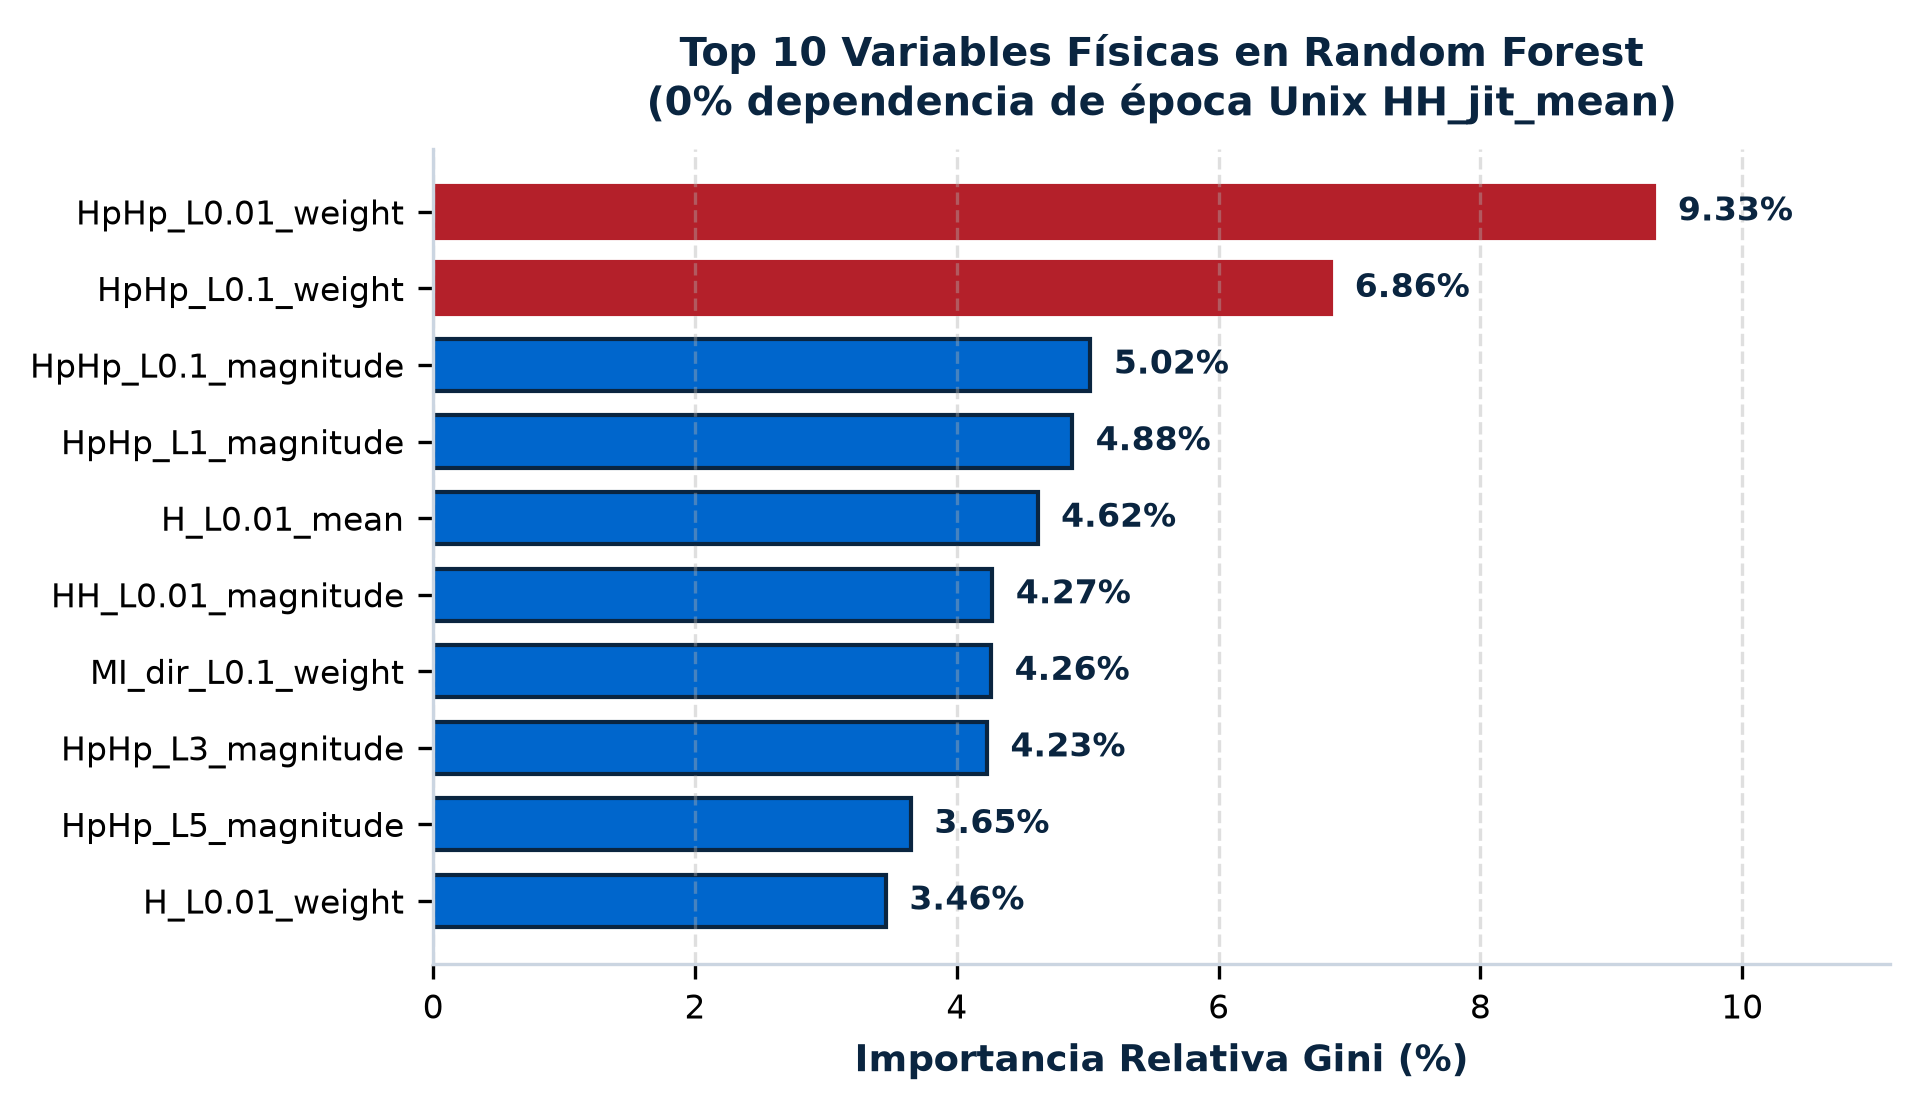
\includegraphics[width=0.82\textwidth]{fig_ppt_importancia_rf.png}%
}{%
  \fbox{\parbox[c][3.5cm][c]{0.8\textwidth}{\centering Top 10 variables físicas en Random Forest tras sanitización}}%
}
\caption{Importancia relativa Gini de las diez principales variables físicas en Random Forest tras la sanitización de la época Unix en \texttt{HH\_jit}.}
\label{fig:importancia-rf}
\end{figure}

\subsubsection{Evaluación por dispositivo externo en rotación ciega (Protocolo 6/2/1)}
La Tabla~\ref{tab:resultados-621} resume los promedios no ponderados sobre los nueve dispositivos excluidos del protocolo riguroso 6/2/1. Se reportan simultáneamente el umbral fijo ($0{,}5$) y el umbral ajustado en los dos dispositivos de calibración ($\text{FPR} \le 0{,}1\%$) para separar la dificultad intrínseca de los datos respecto del efecto del ajuste del umbral.

\begin{table}[H]
\centering\small
\caption{Evaluación por dispositivo excluido (Protocolo 6/2/1: seis dispositivos de ajuste, dos de calibración y uno de prueba).}
\label{tab:resultados-621}
\begin{tabularx}{\textwidth}{l l c c c X}
\toprule
\textbf{Modelo} & \textbf{Umbral} & \textbf{F1 medio} & \textbf{FPR medio} & \textbf{Peor FPR} & \textbf{Menor recall} \\
\midrule
Regresión Logística (LR) & Fijo 0,5 & 0,9933 & 2,42\% & 16,55\% & 99,45\% \\
Regresión Logística (LR) & Ajustado & 0,8007 & 0,04\% & 0,35\% & 22,62\% \\
\textbf{Random Forest (RF)} & Fijo 0,5 & \textbf{0,9998} & 0,05\% & 0,25\% & 99,95\% \\
\textbf{Random Forest (RF)} & \textbf{Ajustado} & \textbf{0,9995} & \textbf{0,14\%} & \textbf{0,51\%} & \textbf{99,95\%} \\
Gradient Boosting (GB) & Fijo 0,5 & 0,9934 & 1,87\% & 9,10\% & 99,95\% \\
Gradient Boosting (GB) & Ajustado & 0,9452 & 2,95\% & 16,55\% & 60,00\% \\
\bottomrule
\end{tabularx}
\end{table}
{\footnotesize Fuente: elaboración propia a partir de \texttt{experiments/rigorous\_v1/summary.csv}. Las métricas no se mezclan con el LODO histórico 8/1.}

Al imponer un presupuesto estricto de falsas alarmas ($\text{FPR} \le 0{,}1\%$), la Regresión Logística degrada severamente su detección (F1 medio 0,8007 y menor recall 22,62\%) y Gradient Boosting cae a F1 medio 0,9452 (menor recall 60,00\% y peor FPR 16,55\%). En contraste, Random Forest conserva un F1 medio de 0,9995, FPR medio de 0,14\% y peor recall de 99,95\% frente a dispositivos nunca vistos con familias conocidas.

\subsubsection{Exclusión total de familias (Zero-Day) y ablaciones de características}
La Tabla~\ref{tab:zeroday} presenta los 16 escenarios de exclusión conjunta de familia y dispositivo sobre Random Forest, mientras que la Tabla~\ref{tab:ablaciones} y la Figura~\ref{fig:zeroday-caida} sintetizan el impacto de las ablaciones y la caída real ante familias inéditas.

\begin{table}[H]
\centering\scriptsize
\caption{Evaluación de familia y dispositivo nunca vistos (\textit{Zero-Day}) en Random Forest (16 escenarios).}
\label{tab:zeroday}
\begin{tabularx}{\textwidth}{l c c c c c c}
\toprule
\textbf{Familia excluida} & \textbf{Dispositivo} & \textbf{F1 (umbral 0,5)} & \textbf{F1 (ajustado)} & \textbf{Recall (ajustado)} & \textbf{FP} & \textbf{FN (de 2.000)} \\
\midrule
BASHLITE (\texttt{gafgyt}) & 1 (Danmini) & 0,7257 & 1,0000 & 100,00\% & 0 & 0 \\
Mirai & 1 (Danmini) & 0,8907 & 0,8907 & 80,30\% & 0 & 394 \\
BASHLITE (\texttt{gafgyt}) & 2 (Ecobee) & 0,7220 & 0,9906 & 100,00\% & 38 & 0 \\
Mirai & 2 (Ecobee) & 0,9455 & 0,9455 & 89,70\% & 1 & 206 \\
BASHLITE (\texttt{gafgyt}) & 3 (Ennio) & 0,7500 & 0,9995 & 99,95\% & 1 & 1 \\
BASHLITE (\texttt{gafgyt}) & 4 (Philips) & 0,7500 & 0,7500 & 60,00\% & 0 & 800 \\
\textbf{Mirai} & \textbf{4 (Philips)} & \textbf{0,5705} & \textbf{0,5702} & \textbf{39,90\%} & \textbf{1} & \textbf{1.202} \\
BASHLITE (\texttt{gafgyt}) & 5 (Prov.\ 737E) & 0,7500 & 0,7500 & 60,00\% & 0 & 800 \\
Mirai & 5 (Prov.\ 737E) & 0,8546 & 0,8433 & 72,90\% & 0 & 542 \\
\textbf{BASHLITE (\texttt{gafgyt})} & \textbf{6 (Prov.\ 838)} & \textbf{0,6518} & \textbf{0,6537} & \textbf{48,55\%} & \textbf{0} & \textbf{1.029} \\
Mirai & 6 (Prov.\ 838) & 0,8735 & 0,8154 & 68,90\% & 2 & 622 \\
BASHLITE (\texttt{gafgyt}) & 7 (Samsung) & 0,6992 & 0,7009 & 53,95\% & 0 & 921 \\
BASHLITE (\texttt{gafgyt}) & 8 (SH 1002) & 0,6920 & 0,7500 & 60,00\% & 0 & 800 \\
Mirai & 8 (SH 1002) & 0,8318 & 0,9778 & 100,00\% & 91 & 0 \\
BASHLITE (\texttt{gafgyt}) & 9 (SH 1003) & 0,6975 & 0,9973 & 99,95\% & 10 & 1 \\
Mirai & 9 (SH 1003) & 0,8294 & 0,9983 & 100,00\% & 7 & 0 \\
\bottomrule
\end{tabularx}
\end{table}

\begin{table}[H]
\centering\small
\caption{Ablaciones exploratorias de representación de características sobre Random Forest (9 folds 6/2/1).}
\label{tab:ablaciones}
\begin{tabularx}{\textwidth}{X c c c}
\toprule
\textbf{Representación evaluada} & \textbf{F1 externo medio (ajustado)} & \textbf{FPR externo medio} & \textbf{Menor recall} \\
\midrule
\textbf{Sanitizada (sin media/var.\ \texttt{HH\_jit})} & \textbf{0,9995} & \textbf{0,14\%} & \textbf{99,95\%} \\
Jitter crudo (con fuga temporal) & 0,9988 & 0,30\% & 99,98\% \\
Sin variables de peso (\texttt{weight}) & 0,8919 & 0,60\% & 69,00\% \\
Sin ventanas lentas ($\lambda = 0{,}01, 0{,}1$) & 0,8583 & 0,56\% & 29,25\% \\
\bottomrule
\end{tabularx}
\end{table}

\begin{figure}[H]
\centering
\IfFileExists{fig_ppt_zeroday_caida.png}{%
  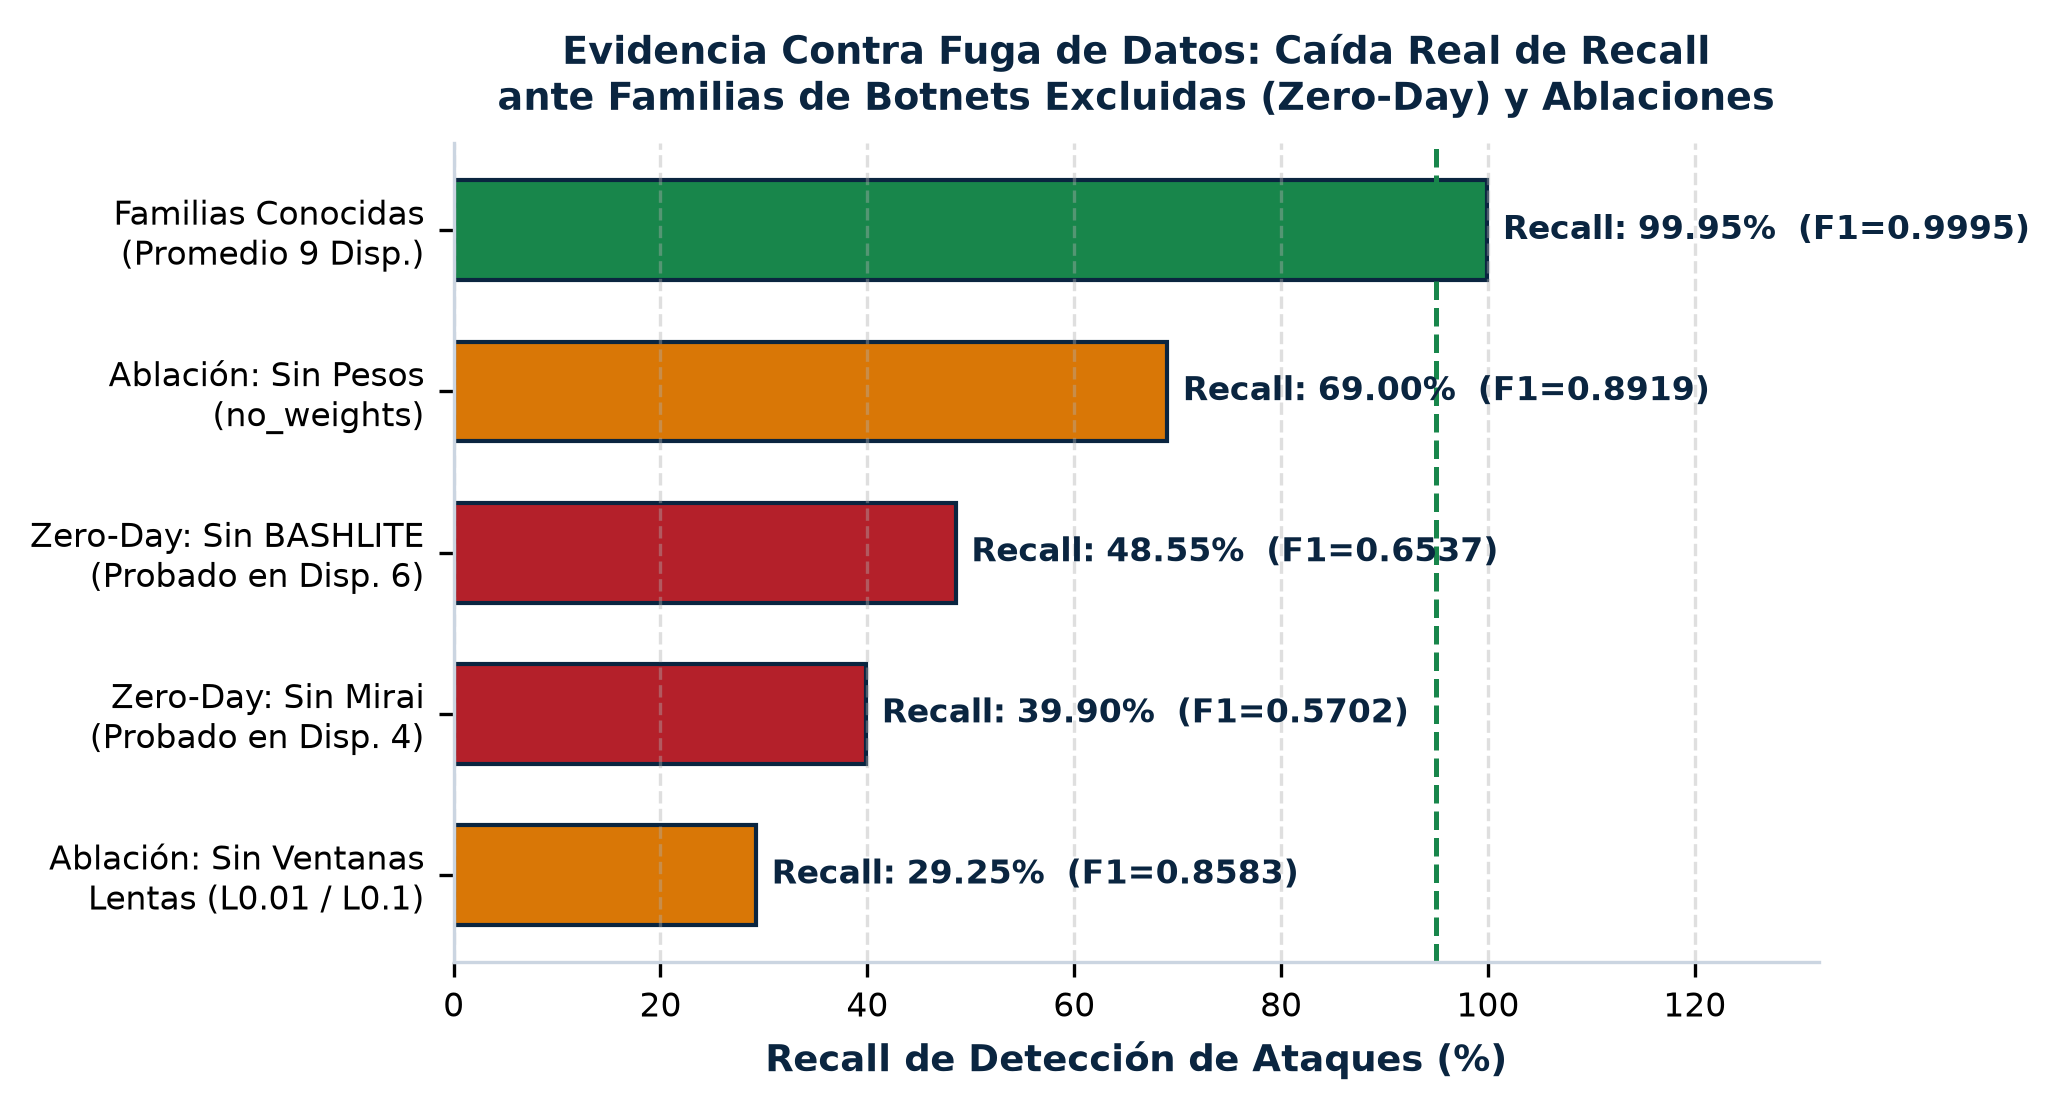
\includegraphics[width=0.86\textwidth]{fig_ppt_zeroday_caida.png}%
}{%
  \fbox{\parbox[c][3.5cm][c]{0.8\textwidth}{\centering Caída de desempeño en ablaciones y exclusión Zero-Day}}%
}
\caption{Contraste entre la detección sobre familias conocidas (99,95\%), la degradación en ablaciones de variables físicas y la caída severa ante exclusión total de familias (\textit{Mirai} en Disp.~4 y \textit{BASHLITE} en Disp.~6).}
\label{fig:zeroday-caida}
\end{figure}

Al excluir por completo Mirai en el dispositivo 4 (Philips Baby Monitor), Random Forest omite 1.202 de 2.000 muestras maliciosas (recall 39,90\%, $F1 = 0{,}5702$). Al excluir BASHLITE en el dispositivo 6 (Provision PT-838), omite 1.029 muestras (recall 48,55\%, $F1 = 0{,}6537$). En las ablaciones, eliminar las ventanas lentas ($\lambda \in \{0{,}01, 0{,}1\}$) desploma el peor recall a 29,25\%, corroborando que el clasificador depende de la acumulación sostenida de paquetes en el tiempo para distinguir ataques volumétricos.

\subsection{Valor, impacto y limitaciones}
La Tabla~\ref{tab:resultados} sintetiza el cumplimiento de los indicadores técnicos, de eficiencia, calidad y ciberseguridad del proyecto.

\begin{table}[H]
\centering\footnotesize
\caption{Resumen consolidado de indicadores, métodos de medición, resultados e interpretación.}
\label{tab:resultados}
\begin{tabularx}{\textwidth}{p{2.7cm} p{3.1cm} p{2.7cm} X}
\toprule
\textbf{Indicador} & \textbf{Método de medición} & \textbf{Resultado} & \textbf{Interpretación} \\
\midrule
F1 y FPR en dispositivo no visto (familias conocidas) & Protocolo ciego 6/2/1 en 9 folds (RF umbral ajustado) & F1 medio 0,9995; FPR medio 0,14\% & Cumple metas ($\ge 0{,}95$ y $\le 1\%$) en dispositivos excluidos para botnets conocidas; supera ampliamente a LR (F1 0,8007). \\
Robustez \textit{Zero-Day} (familia excluida) & Exclusión total de Mirai o BASHLITE en 16 escenarios & Peor recall 39,90\% (Disp.~4) y 48,55\% (Disp.~6) & Falla la meta de 0,95; evidencia ausencia de fuga y demuestra el límite del enfoque puramente supervisado. \\
Eficiencia e inferencia CPU & Cronometraje unitario \texttt{perf\_counter} en CPU convencional & 5,28 ms (RF), 1,03 ms (GB), 0,13 ms (LR) & Cumple meta $\le 10$~ms por vector de características; falta medir latencia extremo a extremo con captura PCAP. \\
Ciberseguridad del prototipo MVP & Verificación JWT \texttt{HS256}, \texttt{SHA-256}, SQLi y Whitelist & 100\% controles verificados en suite & Mitiga manipulación local de modelos, inyección SQL y auto-bloqueo del router en el generador de comandos. \\
Calidad y reproducibilidad & Ejecución de \texttt{unittest} y manifiestos congelados & 25/25 pruebas en verde (0,86 s); 73 exp. & Garantiza contratos de software, disyunción de bloques, onboarding 24h e invitados y trazabilidad completa. \\
\bottomrule
\end{tabularx}
\end{table}

\textbf{Valor e impacto esperado:} para usuarios domésticos y pequeñas organizaciones sin equipos SOC dedicados, el prototipo demuestra la viabilidad de trasladar la inspección desde dispositivos IoT cerrados hacia un punto centralizado de bajo costo, habilitando una estrategia de transformación digital orientada a ciberseguridad proactiva y local (preservando la privacidad al no exportar metadatos a la nube). Sin embargo, el valor observado es de carácter experimental y demostrativo: no sustituye una evaluación con usuarios finales ni acredita operación en producción.

\textbf{Limitaciones y riesgos remanentes:} el muestreo por bloques posicionales no reproduce la prevalencia real de una red doméstica; los datos fueron capturados en 2018 en un único laboratorio; la equivalencia numérica del extractor incremental \texttt{live\_feature\_extractor.py} frente a Kitsune permanece pendiente; y la generación de comandos \texttt{iptables}/\texttt{nftables} no aplica bloqueos físicos sobre un router operacional.

\subsection{Reproducibilidad de los experimentos}
Para reproducir la verificación automatizada y la consola MVP desde el directorio \texttt{proyecto-iot-ml/}:
\begin{verbatim}
.\venv\Scripts\python.exe -m unittest discover -s tests -v
.\venv\Scripts\python.exe -m streamlit run app\app.py
\end{verbatim}
Una ejecución limpia del protocolo riguroso se inicia mediante \texttt{python -m src.models.rigorous --output experiments/nueva}, generando \texttt{protocol\_before\_test.json}, \texttt{environment.json}, \texttt{data\_manifest.json}, \texttt{summary.csv}, \texttt{results.json} y \texttt{RESULTADOS.md}.

% -----------------------------------------------------------------------------
\section{Discusión}

\subsection{Contraste crítico con el estado del arte}
Los resultados obtenidos permiten contextualizar las métricas cercanas al 99,9\% reportadas frecuentemente en la literatura sobre N-BaIoT. Mientras Meidan et al.~\cite{meidan2018} entrenan un \textit{autoencoder} independiente por dispositivo —resolviendo la heterogeneidad a costa de perder escalabilidad ante hardware nuevo— y Hossain e Islam~\cite{hossain2023} o Naeem et al.~\cite{cnnbilstm2025} reportan exactitudes próximas al 99--99,99\% en particiones estáticas intra-dispositivo, nuestra evaluación demuestra que ese desempeño depende críticamente de dos condiciones: que las familias de ataque estén presentes durante el entrenamiento y que las particiones no oculten artefactos temporales.

Al comparar con los estudios que sí evalúan transferencia entre dispositivos, como Wardana et al.~\cite{ensembledn} (exactitud 97,21\% y recall 87,31\%) y Bhilwarawala et al.~\cite{bridge2026} (brechas severas \textit{cross-domain}), nuestros experimentos corroboran la fragilidad de la generalización cuando cambian simultáneamente el fabricante y el vector de ataque. La diferencia fundamental de este trabajo radica en cuantificar explícitamente esa frontera mediante un protocolo sanitizado 6/2/1, mostrando que Random Forest logra generalizar hacia dispositivos nuevos (F1 medio 0,9995 con FPR de 0,14\%) mientras las familias sean conocidas, pero se degrada hasta 39,90\% de recall al introducir una botnet inédita. Conviene reiterar que la literatura de Deep Learning constituye aquí un marco de referencia y no una comparación experimental bajo hardware idéntico.

\subsection{Implicancias de la fuga temporal (\texttt{HH\_jit}), facilidad intrínseca del benchmark y límite supervisado}
El hallazgo de que las columnas \texttt{HH\_jit\_*\_mean} conservaban la época Unix de captura ($\sim 1{,}5\times 10^9$~s) evidencia por qué incorporar la capa de aseguramiento de calidad de CRISP-ML(Q) \cite{studer2021crispmlq} sobre CRISP-DM \cite{chapman2000crispdm} resulta indispensable en ciberseguridad aplicada. Sin esa auditoría, los árboles de decisión podían separar sesiones aprovechando un artefacto cronológico del laboratorio. Una vez saneado el conjunto (verificando cero columnas con magnitudes superiores a $10^7$ entre las 105 variables conservadas) y analizada la importancia Gini (Figura~\ref{fig:importancia-rf}), la ablación sin ventanas lentas (caída del peor recall a 29,25\%) explica físicamente qué aprende el modelo: la persistencia volumétrica de ráfagas DDoS en ventanas de decaimiento lento ($\lambda = 0{,}01$ y $0{,}1$).

Una pregunta crítica frente al F1 medio de 0,9995 en dispositivos externos con familias conocidas es si persiste alguna fuga oculta o si el problema binario dentro de N-BaIoT resulta intrínsecamente separable. La auditoría forense directa sobre las distribuciones crudas de los archivos CSV revela dos factores propios del laboratorio de 2018 que explican estas cifras sin involucrar fuga en el código: (1)~existe una separación física de dos órdenes de magnitud (100$\times$ a 250$\times$) entre equipos benignos en reposo (mediana \texttt{MI\_dir\_L0.01\_weight} entre 29,6 y 115,9 paquetes; \texttt{HpHp\_L0.01\_weight} entre 4,2 y 19,8) y ráfagas de Mirai (3.562 a 8.253 paquetes con \texttt{HpHp\_L0.01\_weight} $= 1{,}0$ constante); y (2)~en las capturas \texttt{gafgyt.tcp} y \texttt{gafgyt.udp}, el uso de \textit{IP-Spoofing} con paquetes fijos de 60~bytes genera vectores casi idénticos entre distintos dispositivos, registrando apenas entre 0,3\% y 0,5\% de filas únicas sobre muestras de 2.000 registros.

En consecuencia, el desempeño realista ante incertidumbre emerge precisamente cuando el problema abandona esa separabilidad artificial: al excluir familias enteras en los 16 escenarios \textit{Zero-Day} (Tabla~\ref{tab:zeroday}, con recall de 39,90\% a 53,95\% y exactitud de 69,9\% a 77,0\%), al clasificar los 10 subtipos crudos de ataque (79,56\% de exactitud), al operar el detector no supervisado \texttt{LOF} (75,60\% de recall) o al enfrentar cámaras multimedia ruidosas en LODO sin calibración (hasta 41,74\% de FPR en el monitor Philips). Esta evidencia descarta contaminación en el protocolo 6/2/1 y justifica tanto la defensa híbrida en tres anillos como el \textit{Modo Aprendizaje 24h} y el \textit{Modo Observación Social} implementados para absorber la entrada de dispositivos nuevos o ráfagas de invitados sin desencadenar falsas alarmas masivas.

\subsection{Calidad, ciberseguridad, eficiencia e impacto sociotécnico}
Desde la perspectiva de ingeniería de software y ciberseguridad, el diseño de doble pipeline desacopla el costo de entrenamiento del entorno de inferencia, garantizando tiempos unitarios de 5,28~ms en CPU sin GPU. La incorporación de controles de defensa en profundidad —autenticación JWT \texttt{HS256} con comparación en tiempo constante, verificación \texttt{SHA-256} previa a la deserialización de artefactos \texttt{joblib}, consultas SQL parametrizadas y lista blanca \textit{Anti-Lockout} combinada con bloqueo Capa~2/Capa~3 (\texttt{IP + MAC})— responde a amenazas reales de operación como el envenenamiento de modelos, la inyección SQL y la denegación de servicio autoinducida por \textit{IP-Spoofing}.

En el plano ético y organizacional, el sistema promueve una protección local que no depende de servicios externos ni inspecciona la carga útil (\textit{payload}) cifrada de las comunicaciones domésticas, reduciendo riesgos de privacidad. No obstante, declarar abiertamente que el prototipo no está autorizado para bloqueo automático en producción evita generar una falsa sensación de seguridad en usuarios no expertos.

\subsection{Amenazas a la validez}
Se reconocen cuatro amenazas principales a la validez externa e interna: (1)~los registros de N-BaIoT provienen de nueve dispositivos comerciales capturados en 2018, por lo que pueden diferir del tráfico moderno (QUIC, HTTP/3, cámaras 4K); (2)~el muestreo balanceado por bloques posicionales no refleja la proporción real de tráfico benigno frente a ataques en operación diaria, impidiendo estimar falsas alarmas por día; (3)~los intervalos de confianza por paquete serían inválidos dada la autocorrelación temporal dentro de una misma ráfaga; y (4)~la consola MVP opera sobre reproducción de vectores CSV precalculados, quedando pendiente la validación numérica del extractor incremental sobre paquetes crudos.

% -----------------------------------------------------------------------------
\section{Conclusiones y trabajo futuro}

\subsection{Síntesis de logros y verificación de objetivos}
El proyecto cumplió íntegramente el ciclo planificado para el semestre 2026-2 (Etapas 1 a 7 / Sprints 1 a 3) bajo la metodología híbrida CRISP-DM / CRISP-ML(Q) y Scrum, integrando evidencia experimental reproducible y un prototipo operativo verificable:
\begin{itemize}
  \item \textbf{Respuesta a la pregunta de investigación:} al separar estrictamente dispositivos de ajuste, calibración y prueba (6/2/1) tras sanear la fuga de época Unix, Random Forest mantiene un desempeño sobresaliente frente a hardware no visto cuando las familias de botnet son conocidas ($F1 = 0{,}9995$, $\text{FPR} = 0{,}14\%$, peor recall 99,95\%), superando holgadamente a Regresión Logística ($F1 = 0{,}8007$) y Gradient Boosting ($F1 = 0{,}9452$). Sin embargo, cuando se excluye una familia completa de ataque, el desempeño supervisado cae de forma crítica (hasta 39,90\% de recall en Mirai/Disp.~4 y 48,55\% en BASHLITE/Disp.~6). Las principales barreras para trasladar estos resultados a una red operacional son la brecha de representatividad temporal (2018), la prevalencia real no evaluada, la calibración de falsas alarmas diarias y la equivalencia pendiente del extractor de paquetes en vivo.
  \item \textbf{Cumplimiento de objetivos específicos:} se consolidó el estado del arte comparando seis referencias clave (OE1); se auditó y saneó el conjunto N-BaIoT completo de 7.062.606 filas sin valores no finitos (OE2); se implementaron y compararon cinco clasificadores supervisados frente al piso trivial \texttt{Dummy} y la línea base lineal, midiendo F1, FPR y latencia CPU $\le 10$~ms (OE3); se ejecutó la validación por dispositivo excluido histórica (LODO 8/1) y el protocolo riguroso 6/2/1 de 73 experimentos con exclusión de familias y ablaciones (OE4); se construyó el emulador controlado de reproducción CSV con inyección dirigida (OE5); y se desplegó el dashboard MVP minimalista en Streamlit con tres anillos, enrutamiento ciego por dispositivo, explicabilidad local Z-Score traducida a lenguaje humano, incorporación dinámica (Modo Aprendizaje 24h e invitados), persistencia SQLite con exportación CSV, autenticación JWT con \textit{rate limiting} y verificación \texttt{SHA-256}, respaldado por 25 pruebas unitarias aprobadas (OE6).
\end{itemize}

\subsection{Trabajo futuro (Continuidad 2027-1)}
En coherencia con las Etapas 8 a 11 del plan anual (Sprints 4 a 7 de Scrum), la continuidad del proyecto se enfoca en cuatro líneas prioritarias para cerrar la brecha entre laboratorio y operación real:
\begin{enumerate}
  \item \textbf{Despliegue en hardware de borde (\textit{Edge Computing}, Etapa 8 / Sprint 4):} portar el motor de inferencia y verificación \texttt{SHA-256} a una Raspberry Pi u otro gateway Linux ARM, midiendo consumo de memoria, CPU y latencia extremo a extremo.
  \item \textbf{Captura en vivo y certificación del extractor $O(1)$ (Etapa 9 / Sprint 5):} conectar \texttt{live\_feature\_extractor.py} a tráfico capturado por \textit{Port Mirroring} (\texttt{libpcap}), certificando su equivalencia numérica con Kitsune y añadiendo poda de memoria para operación 24/7.
  \item \textbf{Evaluación prolongada de falsas alarmas en red doméstica real (Etapa 10 / Sprint 6):} medir FPR diaria bajo uso cotidiano (videollamadas, \textit{streaming} y dispositivos modernos) y validar la ejecución controlada con reversión automática de reglas \texttt{iptables}/\texttt{nftables} en OpenWrt.
  \item \textbf{Evolución no supervisada para amenazas \textit{Zero-Day} (Etapa 11 / Sprint 7):} entrenar y cuantizar un \textit{autoencoder} liviano para CPU de borde como evolución del Anillo~3, evaluando si recupera la tasa de detección en los escenarios donde el modelo supervisado descendió a 39,90--48,55\%.
\end{enumerate}

\clearpage
\phantomsection
\addcontentsline{toc}{section}{Referencias}
\bibliographystyle{unsrt}
\bibliography{references}

\appendix
\section{Declaración de uso de inteligencia artificial}
Se utilizaron asistentes de inteligencia artificial generativa (Claude, Gemini y ChatGPT/Codex) como apoyo para la estructuración documental en LaTeX, revisión y refactorización de código modular, diseño de pruebas unitarias, auditoría metodológica contra fuga de datos y síntesis de tablas y gráficos reproducibles. Cada código, métrica y cita bibliográfica fue ejecutada, verificada y auditada localmente sobre los scripts y archivos de resultados del repositorio (\texttt{models\_registry/}, \texttt{experiments/rigorous\_v1/} y \texttt{tests/}). El estudiante asume la responsabilidad íntegra por la exactitud técnica, la interpretación científica, la originalidad del trabajo y el dominio demostrado en las defensas orales. No se ingresaron credenciales reales ni capturas privadas de redes domésticas en herramientas externas.

\section{Contribución individual}
El proyecto fue desarrollado íntegramente de forma individual, correspondiendo la totalidad del diseño, implementación, experimentación, documentación y defensa al autor indicado en la Tabla~\ref{tab:contribucion}.

\begin{table}[H]
\centering
\caption{Contribución individual del integrante.}
\label{tab:contribucion}
\footnotesize
\begin{tabularx}{\textwidth}{p{0.20\textwidth}p{0.46\textwidth}X}
\toprule
\textbf{Integrante} & \textbf{Responsabilidades / contribuciones} & \textbf{Evidencias} \\
\midrule
\students & Formulación del problema y estado del arte; definición de metodología híbrida CRISP-DM/CRISP-ML(Q) + Scrum; auditoría completa de 89 CSV (7,06M filas) y saneamiento \texttt{HH\_jit}; desarrollo del pipeline offline (5 clasificadores, 3 anillos y protocolo riguroso 6/2/1 de 73 experimentos); implementación del MVP en Streamlit (JWT, \texttt{SHA-256}, SQLite, generador firewall y enrutamiento ciego); suite de 25 pruebas unitarias; redacción del paper final, diseño del póster, presentación y portafolio. & Repositorio GitHub \url{https://github.com/FelipeNVR/proyecto-iot-ml}, directorio \texttt{proyecto-iot-ml/}, \texttt{experiments/rigorous\_v1/}, \texttt{models\_registry/}, suite \texttt{tests/} (25/25 OK), \texttt{main.tex}, \texttt{poster\_E3.tex}, \texttt{presentacion\_E3.tex} y \texttt{PORTAFOLIO\_E3\_CINF200.md}. \\
\bottomrule
\end{tabularx}
\end{table}

\section{Evidencias complementarias y artefactos del proyecto}
La Tabla~\ref{tab:evidencias} consolida el inventario de artefactos técnicos, código fuente, material gráfico y documentación reproducible generados en el proyecto.

\begin{table}[H]
\centering
\caption{Inventario de evidencias técnicas y artefactos complementarios.}
\label{tab:evidencias}
\footnotesize
\begin{tabularx}{\textwidth}{p{0.25\textwidth}p{0.31\textwidth}X}
\toprule
\textbf{Artefacto} & \textbf{Ubicación / enlace} & \textbf{Descripción y estado} \\
\midrule
Prototipo MVP y código fuente & \url{https://github.com/FelipeNVR/proyecto-iot-ml} (\texttt{proyecto-iot-ml/}) & Consola Streamlit operativa (\texttt{app/app.py}), motor de 3 anillos, 9 folds ciegos 6/2/1, modo aprendizaje 24h e invitados (\texttt{device\_onboarding.py}), 73 experimentos y 25/25 pruebas unitarias aprobadas. \\
Póster científico & \texttt{poster\_E3.tex} (PDF A0) & Póster científico profesional con problema, metodología híbrida CRISP-DM/CRISP-ML(Q) + Scrum, arquitectura, resultados 6/2/1, caída Zero-Day y conclusiones. \\
Presentación de soporte & \texttt{presentacion\_E3.tex} (PDF 16:9) & Presentación ejecutiva complementaria con gráficos de alta resolución (300 DPI), discusión crítica y demostración guiada. \\
Portafolio técnico & \texttt{PORTAFOLIO\_E3\_CINF200.md} y repositorio GitHub & Índice trazable con el inventario completo de fuentes, planes, código, experimentos reproducibles y declaraciones de autoría. \\
Demostración interactiva & Consola local (\texttt{http://localhost:8501}) & Demostración en vivo de autenticación JWT, tráfico normal, inyección ciega por dispositivo excluido (\texttt{device\_X\_rf}), causa raíz Z-Score y generación de reglas \texttt{iptables}. \\
\bottomrule
\end{tabularx}
\end{table}

\end{document}
